\chapter{Extending Reinforcement Learning in Diffusion Models}

\section{Introduction}

\ca{La intención de este capítulo es que sea autocontenido y no dependa de los capítulos anteriores. Sin embargo, dentro del contexto de la tesis, igual
es como redundante la introducción a este nivel. Considerando que hay un
capítulo introductorio que debiera ser leído antes de este y contener el
objetivo de esta tesis. \textbf{Entonces}, agregar un disclaimer sobre que la introducción esta repetida y que se puede omitir su lectura, o derechamente
remover la introducción de este capítulo.}

Reinforcement learning has shown the capacity to orchestrate or align highly complex generative models, which often proves impossible using a supervised learning objective such as matching distribution \ca{referencia ChatGPT?}. \ca{(suavizar esta transición)} Constructing agents based on generative models can be seen as a user-model interface endeavor, an intriguing line of exploration from the perspective of human-computer interaction (HCI) \ca{Agregar referencia.}. While reinforcement learning is not a cheap or intuitive approach, it offers flexibility and simplicity by optimizing a reward. Regarding the cost of sampling, highly capable generative models such as LLMs and diffusion models have fostered research efforts to reduce inference times for sample generation (inference as a first citizen). These advances make it more appealing to construct agents atop these models. \\

\noindent In this work, we propose several extensions to the formulation of the diffusion process as a sequential decision-making process, specifically regarding how to exploit the information from the intermediate state rewards rather than only using the final trajectory outcome. Based on the \textit{insights} of the reward signal behavior in sample generation, we propose methods based on the challenge classifier guidance techniques from the diffusion model literature. Moreover, we explore the use of baseline functions, a technique known to reduce the variance of the gradient estimator when using Monte Carlo estimation \cite{mohamed2020monte}, without introducing bias into the estimator. We compare the implementation of these extensions to the DDPO algorithm \cite{black2023training} on which our formulation is based, on the same \textit{downstream tasks} used in this work, such as JPEG compressibility and incompressibility, and aesthetic quality. \\

\noindent Our contributions extend the existing framework of the diffusion process by exploiting the informative intermediate state rewards rather than solely relying on the final trajectory outcome. We analyze the reward signal dynamics throughout the denoising process using a collection of sample trajectories from the \textit{google/ddpm-celebahq-256} model. Additionally, we propose extended reward functions that incorporate further information beyond the final sample, alongside the introduction of baseline functions during RL training. Model checkpoints are provided for each of the proposed methods, allowing for further exploration and comparison (see Appendix~\ref{appendix:implementation}). \\

%Code: \href{https://github.com/alcazar90/ddpo-celebahq}{https://github.com/alcazar90/ddpo-celebahq}

% Visual comparison between pretrained and ckpts fintuned with DDPO
\begin{figure}[ht]
  \centering
  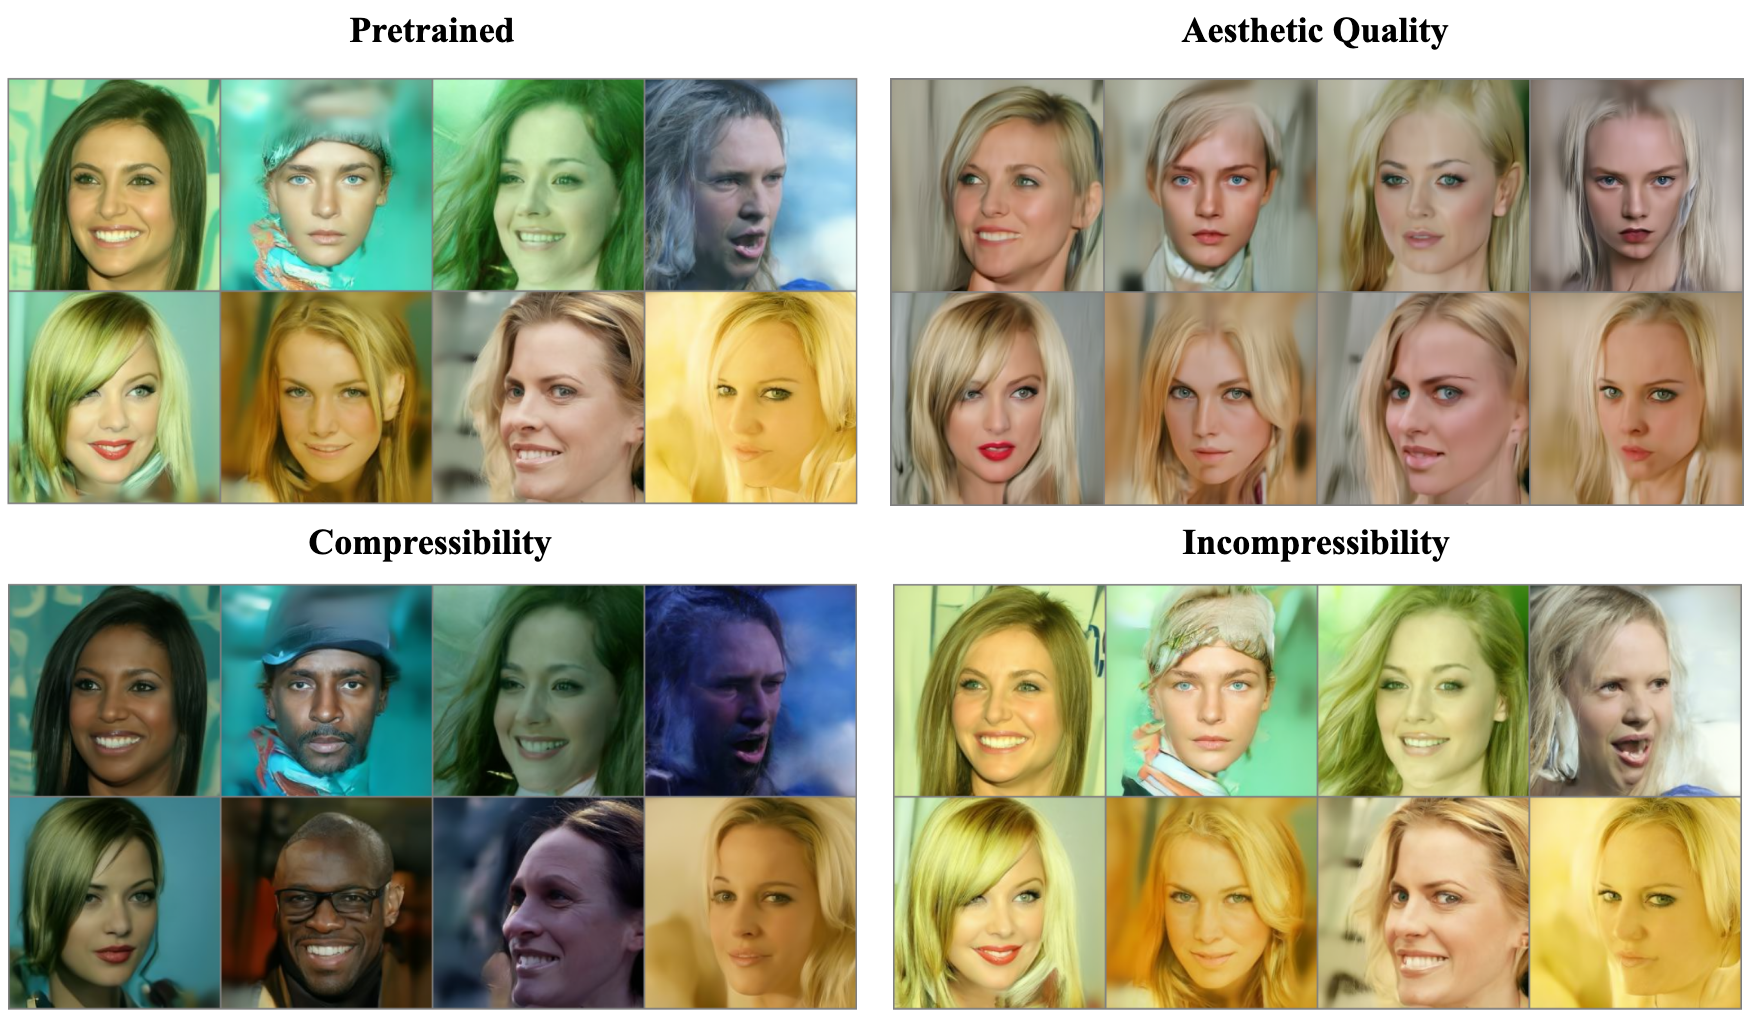
\includegraphics[scale=0.72]{img/results/visual-comparison-results-200dpi.png}
  \vspace{-4pt}  % reduce space between caption and figure
    \captionsetup{width=\textwidth} % set the width of the caption
    \caption{\textbf{DDPM pretrained model's samples vs DDPO finetuned samples.} Qualitative depiction of the effects of RL finetuning on different reward functions. Additional samples in the Appendix~\ref{appendix:additional-samples}.}
    \label{fig:visual-comparison-ddpo}
\end{figure}

\section{Related Work}

\noindent\textbf{Diffusion Models.} Muy breve y referenciar capítulo de background.\\

\noindent\textbf{Reinforcement Learning.} Muy breve y referenciar capítulo de background.\\

\noindent\textbf{Reinforcement Learning from Human Feedback (RLHF).} Recently the attention to use human feedback in reinforcement learning has increased \cite{kaufmann2023survey}. The core idea is to capture the human feedback into a reward model that can be used to train the policy that dictates the agent's behaviour. The benefits it's to allow different types of feedback, such as binary, continuous, or even more complex signals that can be used to train in a supervised learning fashion. Then, instead of design the reward function---or use feature engineering---we can gives the agent access to the reward model to obtain the neccessary information to label trajectories and optimize its behaviour to learn the task. \\

\noindent\textbf{Reinforcement learning \& Diffusion models.} Citar trabajos de Schulman \citep{schulman2015trust} y \citep{schulman2017proximal}. The former work extend a theoretical lower bound that works for policy update, original present for the case of mixture policies (something between $\pi_{old}$ and $\pi`$), and now adapted to stochastic policies. They introduce a distance measure between policies: total variation divergence. In the following section, we will detailed more the policy optimization approach for finetuned diffusiono models with RL.\\

\section{Diffusion Model as Sequential Decision making Process}\label{sec:diffusion-model-mdp}

% Diffusion Model as MDP
\begin{figure}[ht]
  \centering
  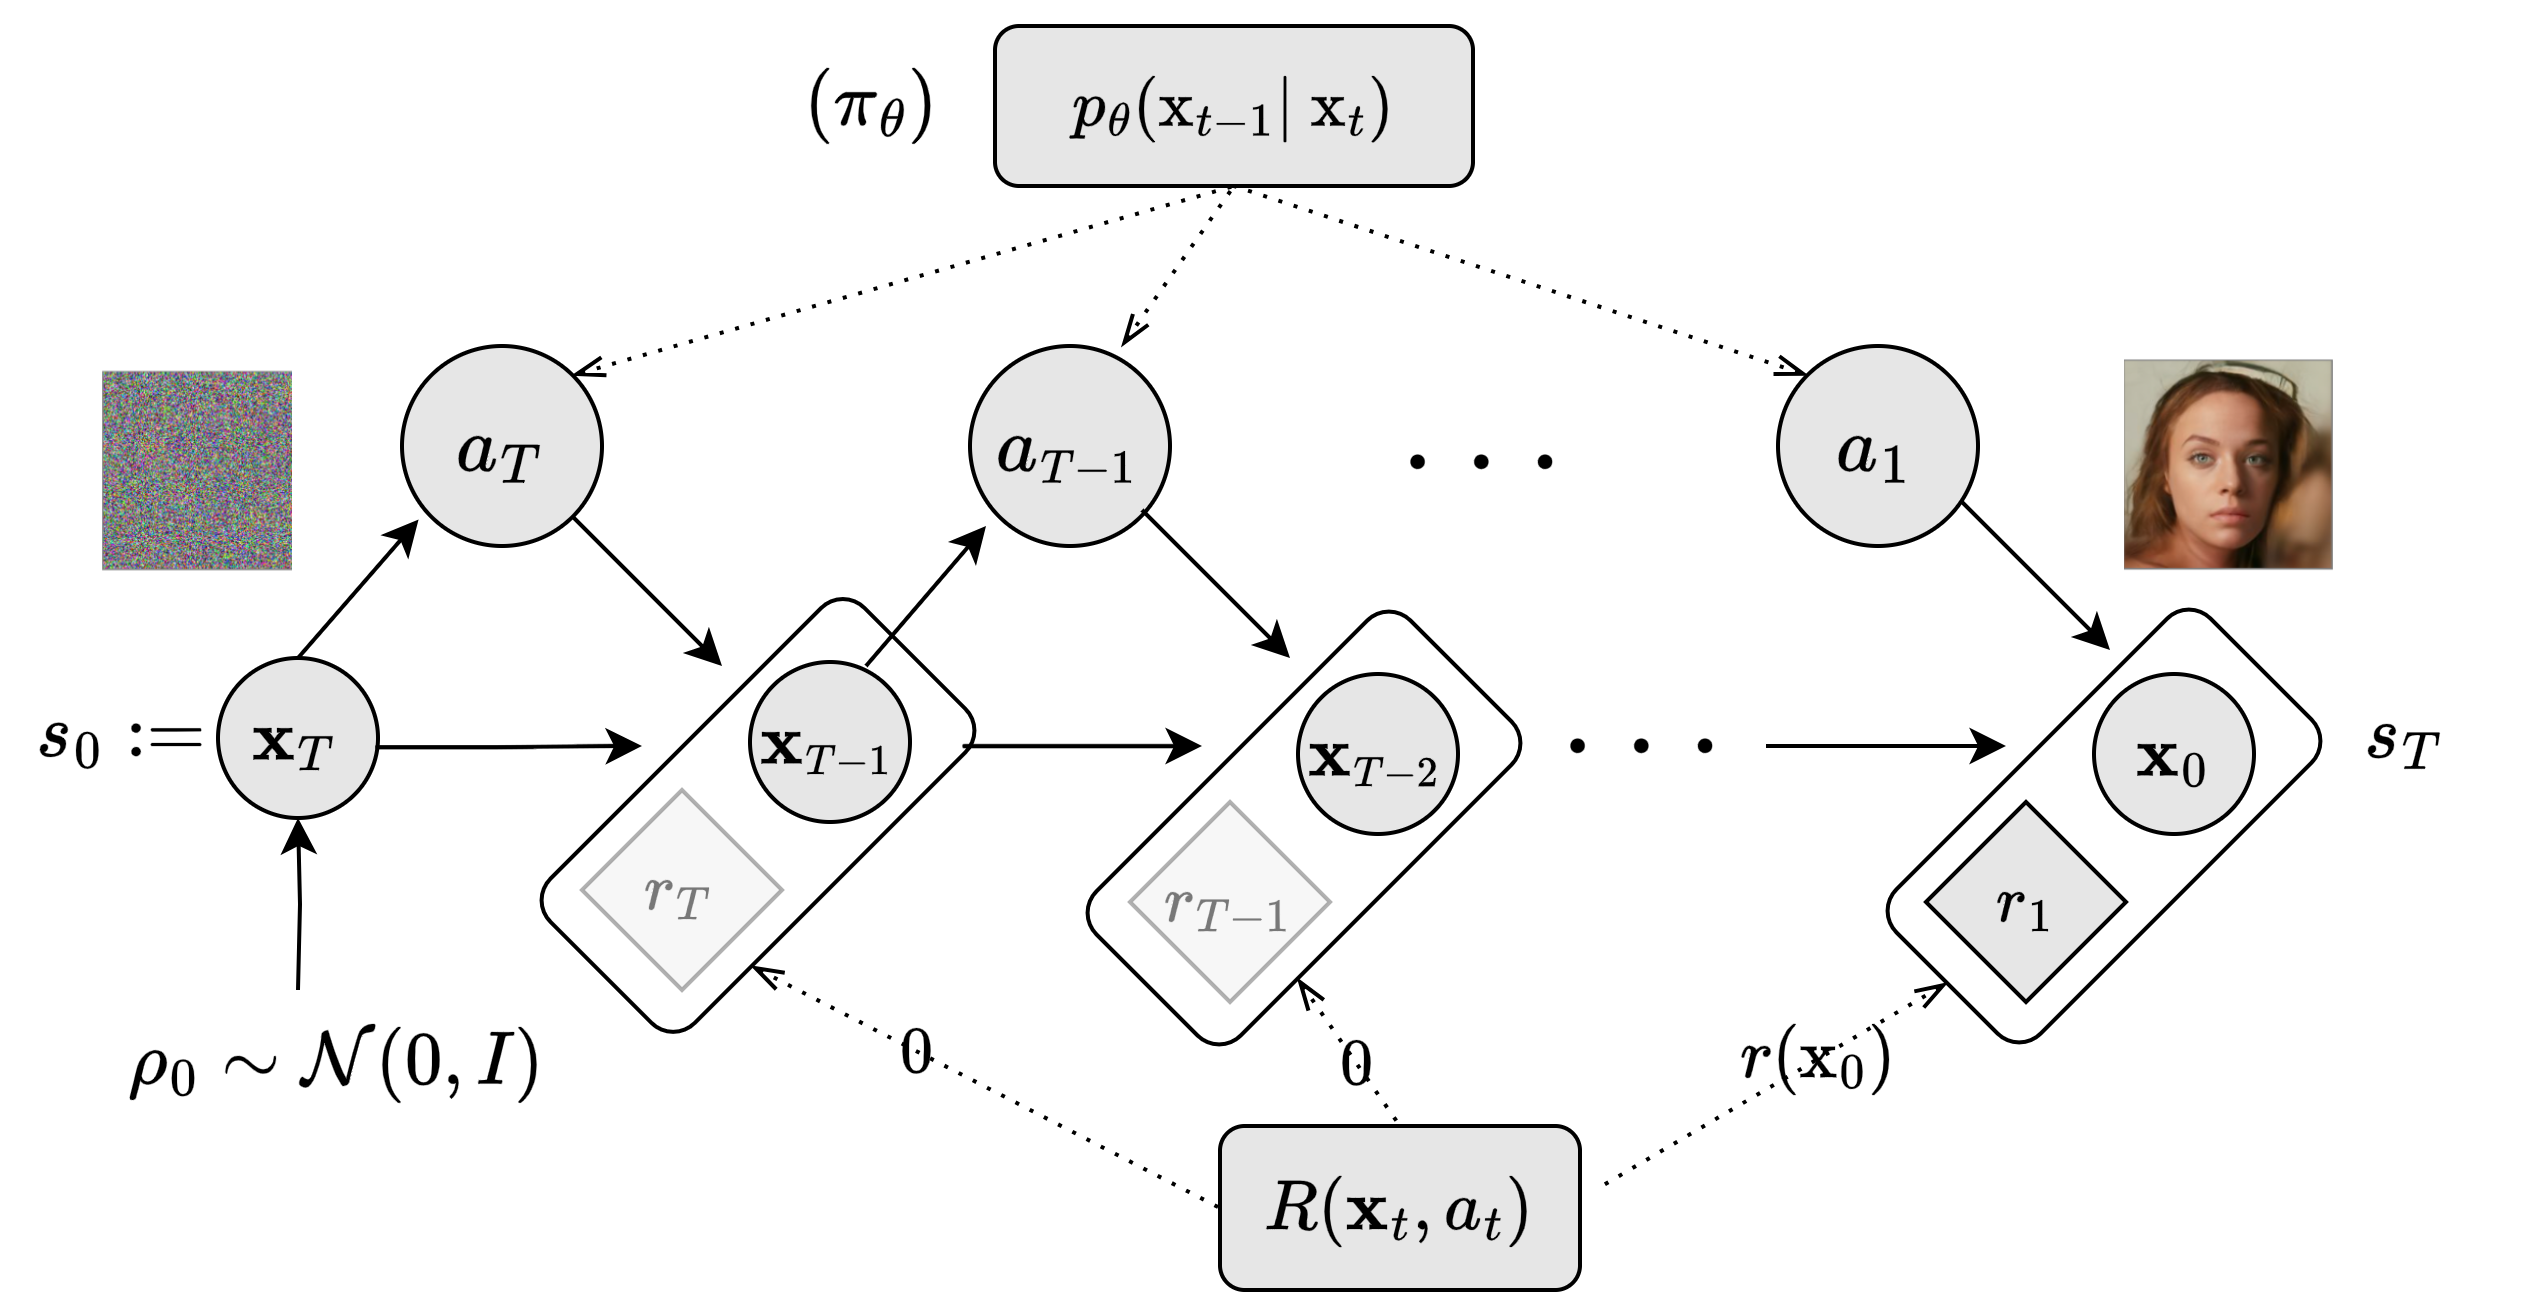
\includegraphics[scale=0.85]{img/results/diffusion-model-MDP.png}
  \vspace{-4pt}  % reduce space between caption and figure
    \captionsetup{width=\textwidth} % set the width of the caption
    \caption{\textbf{Diffusion model as a sequential decision-making process.} The policy $\pi_{\theta}:=p_{\theta}(\mathrm{x}_{t-1} | \mathrm{x}_{t})$  takes denoising decisions from pure noise to the final sample $\mathrm{x}_0$ through the entire backward process $\tau=\mathrm{x}_{T:0}$.}
  \label{fig:diffusion-model-mdp}
\end{figure}

% agregar función de reward...
We consider the denoising diffusion policy optimization (DDPO) formulation \citep{black2023training} as a starting point. The initial state of the Markov decision process,
$\mathrm{s}_{0}$, is sampling from an isotropic
Gaussian distribution 
$\rho_{0}\sim\mathcal{N}(0, I)$, corresponding to the
noise $\mathrm{x}_{T}$ at the beginning of the
diffusion backward process as shown in Figure~\ref{fig:diffusion-model-mdp}, where the sample
generation starts. 
Then, a \textit{denoising} neural network $p_{\theta}$
is used to directly estimate $\mathrm{x}_{t-1}$ at
timestep $t$ (or indirectly by
estimating the noise $\hat{\epsilon}_{t}$) and is
treated as a policy $\pi_{\theta}(a_{t}, s_{t})$. The policy describes how an agent---\textit{via its denoising actions $a_{t}$}---moves from a noisy
step to a less noisy one (i.e. 
$a_t: \mathrm{x}_{t} \rightarrow \mathrm{x}_{t-1}$) until arrives to a terminal state $s_T$, where the sample $\mathrm{x}_{0}$ is generated. \\

\noindent In this framework, we can optimize the diffusion
model parameters $\theta$ directly via policy
gradient estimation to maximize any arbitrary
scalar-reward signal over the sample $\mathrm{x}_{0}$.
In other words, the agent learns how to denoise trajectories to maximize the expected reward using the following objective:

\begin{equation}\label{difusion-rl-objective-1}
  \mathcal{J}_{\text{DDRL}}(\theta)
  = \mathbb{E}_{\mathrm{c}\sim p(\mathrm{c}),  \mathrm{x}_{0}\sim p_{\theta}(\mathrm{x}_{0}|\mathrm{c})}[ r(\mathrm{x}_{0}, \mathrm{c})]
\end{equation}

\noindent A relevant aspect of this formulation is that the reward $R(s_{t}, a_{t})$
only provides information about the final sample $\mathrm{x}_{0}$, giving zero
reward to each non-terminal state, or $\mathrm{x}_{t}$ where $t\neq0$ as it is
depicted in Figure~\ref{fig:diffusion-model-mdp}. Additionally, DDPO-based methods propose two ways to compute the gradients: (i) via a score function method, also known as REINFORCE, and (ii) using importance sampling to optimize a surrogate objective \cite{schulman2015trust, schulman2017proximal}. This second approach, denoted $\text{DDPO}_{\text{IS}}$ in Eq.~\eqref{eqn:ddpo-is-objective}, is used as benchmark in this work to compare the proposed method.\footnote{When we refer to DDPO from here on without specifying, it is DDPO with importance sampling (aka PPO algorithm \citep{schulman2017proximal}).} 
% agregar objetivo DDPO_{SF}
%\begin{equation}\label{eqn:ddpo-sf-objective}
%  (\text{DDPO}_{\text{SF}})~~ \nabla_{\theta}\mathcal{J} = \mathbb{E}_{\mathrm{x}_{T:0}\sim p_{\theta}} \bigg[\sum_{t=0}^{T}\nabla_{\theta}\log p_{\theta}(\mathrm{x_{t-1}|\mathrm{x}_t}) r(\mathrm{x}_{0})\bigg]
%\end{equation}
% agregar objetivo DDPO_{IS}
\begin{equation}\label{eqn:ddpo-is-objective}
  (\text{DDPO}_{\text{IS}})~~ \nabla_{\theta}\mathcal{J} = \mathbb{E}_{\mathrm{x}_{T:0}\sim p_{\theta_{\text{old}}}} \bigg[\sum_{t=0}^{T}\frac{p_{\theta}(\mathrm{x}_{t-1}|\mathrm{x}_{t})}{p_{\theta_{\text{old}}}(\mathrm{x}_{t-1}|\mathrm{x}_{t})}\nabla_{\theta}\log p_{\theta}(\mathrm{x_{t-1}|\mathrm{x}_t}) r(\mathrm{x}_{0})\bigg]
\end{equation}

\noindent It is straightforward to compute $\log p_{\theta}$ considering that
$p_{\theta}$ is a conditional gaussian distribution 
$\mathcal{N}(f_{\theta}(\mathrm{x}_{t}) | \mathrm{x}_{t-1}, \alpha)$, where
$f_{\theta}$ is a neural network such as U-net architecture parameterized by $\theta$. \ca{Ser más riguroso en el uso de $p_{\theta}$ como $f_{\theta}$ para aproximar la media, dado que más adelante se usa $f_{\theta}$ con la notación de DDIM para aproximar los estados intermedios a la muestra final. Agregar cómo despejar la formula para obtener el código?}

\section{Extending RL in diffusion models}\label{sec:extending-methodology}

\ca{GAE y extender PPO como actor-critic usando value function es una formulación más general que DDPO. ¿Porqué no usarla? Hay unas implementaciones
actor-critic con PPO, no creo que esto sea necesariamente GAE, pero entender
la diferencia. Eso si, considerar siempre que la policy network se ajusta para
y el rol del value network es mejorar la performance de la actualización de 
gradientes. Por otro lado, la justificación de usar GAE es que se incorpora
los reward de la trayectoria completa, lo cual es una forma de obtener tanto
el beneficio del baseline con value function pero también de incorporar la
información que puede tener el reward en pasos intermedios.}

Simplifying the problem and ignoring the context raise from conditional generative models such as text-to-image, instead we assume an unconditional model free of context. Following...
\begin{equation}\label{difusion-rl-objective-2}
  \mathcal{J}_{\text{DDRL}}(\theta)
  = \mathbb{E}_{\mathrm{x}_{0}\sim p_{\theta}(\mathrm{x}_{T:0})}[R(\mathrm{x}_{T:0})]
\end{equation}

Based on the summarization of policy gradients in \cite{schulman2015high} we can see the design decision to extend reinforcement learning, these are non excluyentes...
\begin{equation}\label{eqn:general-pg-estimation-form}
  \nabla_{\theta}\mathcal{J}(\theta) = \mathbb{E}\bigg[\sum_{t=0}^{\infty}\Psi_{t}\nabla_{\theta}\log\pi_{\theta}(a_{t}|s_{t}) \bigg]
\end{equation}
En la Figure~\ref{fig:diffusion-model-mdp}, el reward signal $\Psi_{t}$ es cero para todo $t\neq0$. Por lo tanto, el objetivo de RL se reduce a maximizar el reward en el estado terminal $\mathrm{x}_{0}$. Considering alternatives
to extend the reward signal summarize in \textit{High-Dimensional Continuous Control Using Generalized Advantage Estimation} \cite{schulman2015high}, we propose the following formulations.

\begin{equation}
  g = \mathbb{E} \left[ \sum_{t=0}^{\infty} \Psi_t \nabla_\theta \log \pi_\theta (a_t | s_t) \right],
  \end{equation}
  
  where $\Psi_t$ may be one of the following:

  \begin{multicols}{2}
    \begin{enumerate}
        \item $\sum_{t=0}^{\infty} r_t$: total reward of the trajectory.
        \item $\sum_{t'=t}^{\infty} r_{t'}$: reward following action $a_t$.
        \item $\sum_{t'=t}^{\infty} r_{t'} - b(s_t)$: baselined version of previous formula.
        \item $Q^{\pi}(s_t, a_t)$: state-action value function.
        \item $A^{\pi}(s_t, a_t)$: advantage function.
        \item $r_t + V^{\pi}(s_{t+1}) - V^{\pi}(s_t)$: TD residual.
    \end{enumerate}
  \end{multicols}

  The latter formulas use the definitions
  
  \begin{equation}
  V^{\pi}(s_t) := \mathbb{E}_{s_{t+1:\infty}, a_{t:\infty}} \left[ \sum_{l=0}^{\infty} r_{t+l} \right]
  \end{equation}
  
  \begin{equation}
  Q^{\pi}(s_t, a_t) := \mathbb{E}_{s_{t+1:\infty}, a_{t+1:\infty}} \left[ \sum_{l=0}^{\infty} r_{t+l} \right]
  \end{equation}
  
  \begin{equation}
  A^{\pi}(s_t, a_t) := Q^{\pi}(s_t, a_t) - V^{\pi}(s_t) \quad \text{(Advantage function).}
  \end{equation}


\ca{\textbf{Importante:} Si se encuentra implementación de GAE, todas las
posibilidades anteriores son consideradas por este ``estimador'', por tanto,
no sería necesario (i) consiederar cual usar o es más apropiada, (ii) 
implementar más de una (en honor al tiempo), y (iii) considerar lo del baseline
como una extensión aparte de considerar el reward de la trayectoria, esta
formulación tenemos eso gratis.}


\subsection{MaDI: a masker to turn off non-informative pixels}

\ca{Francamente no se si haya tiempo para esto o tiene sentido. Se puede agregar en trabajo futuro y asociar con apagar pixes intermedios, o una forma de "estimación" del reward intermedio, o regularización.}

% Reward signal during samples trajectories 
\begin{figure}[ht]
  \centering
  \begin{minipage}{0.5\textwidth}
      \centering
      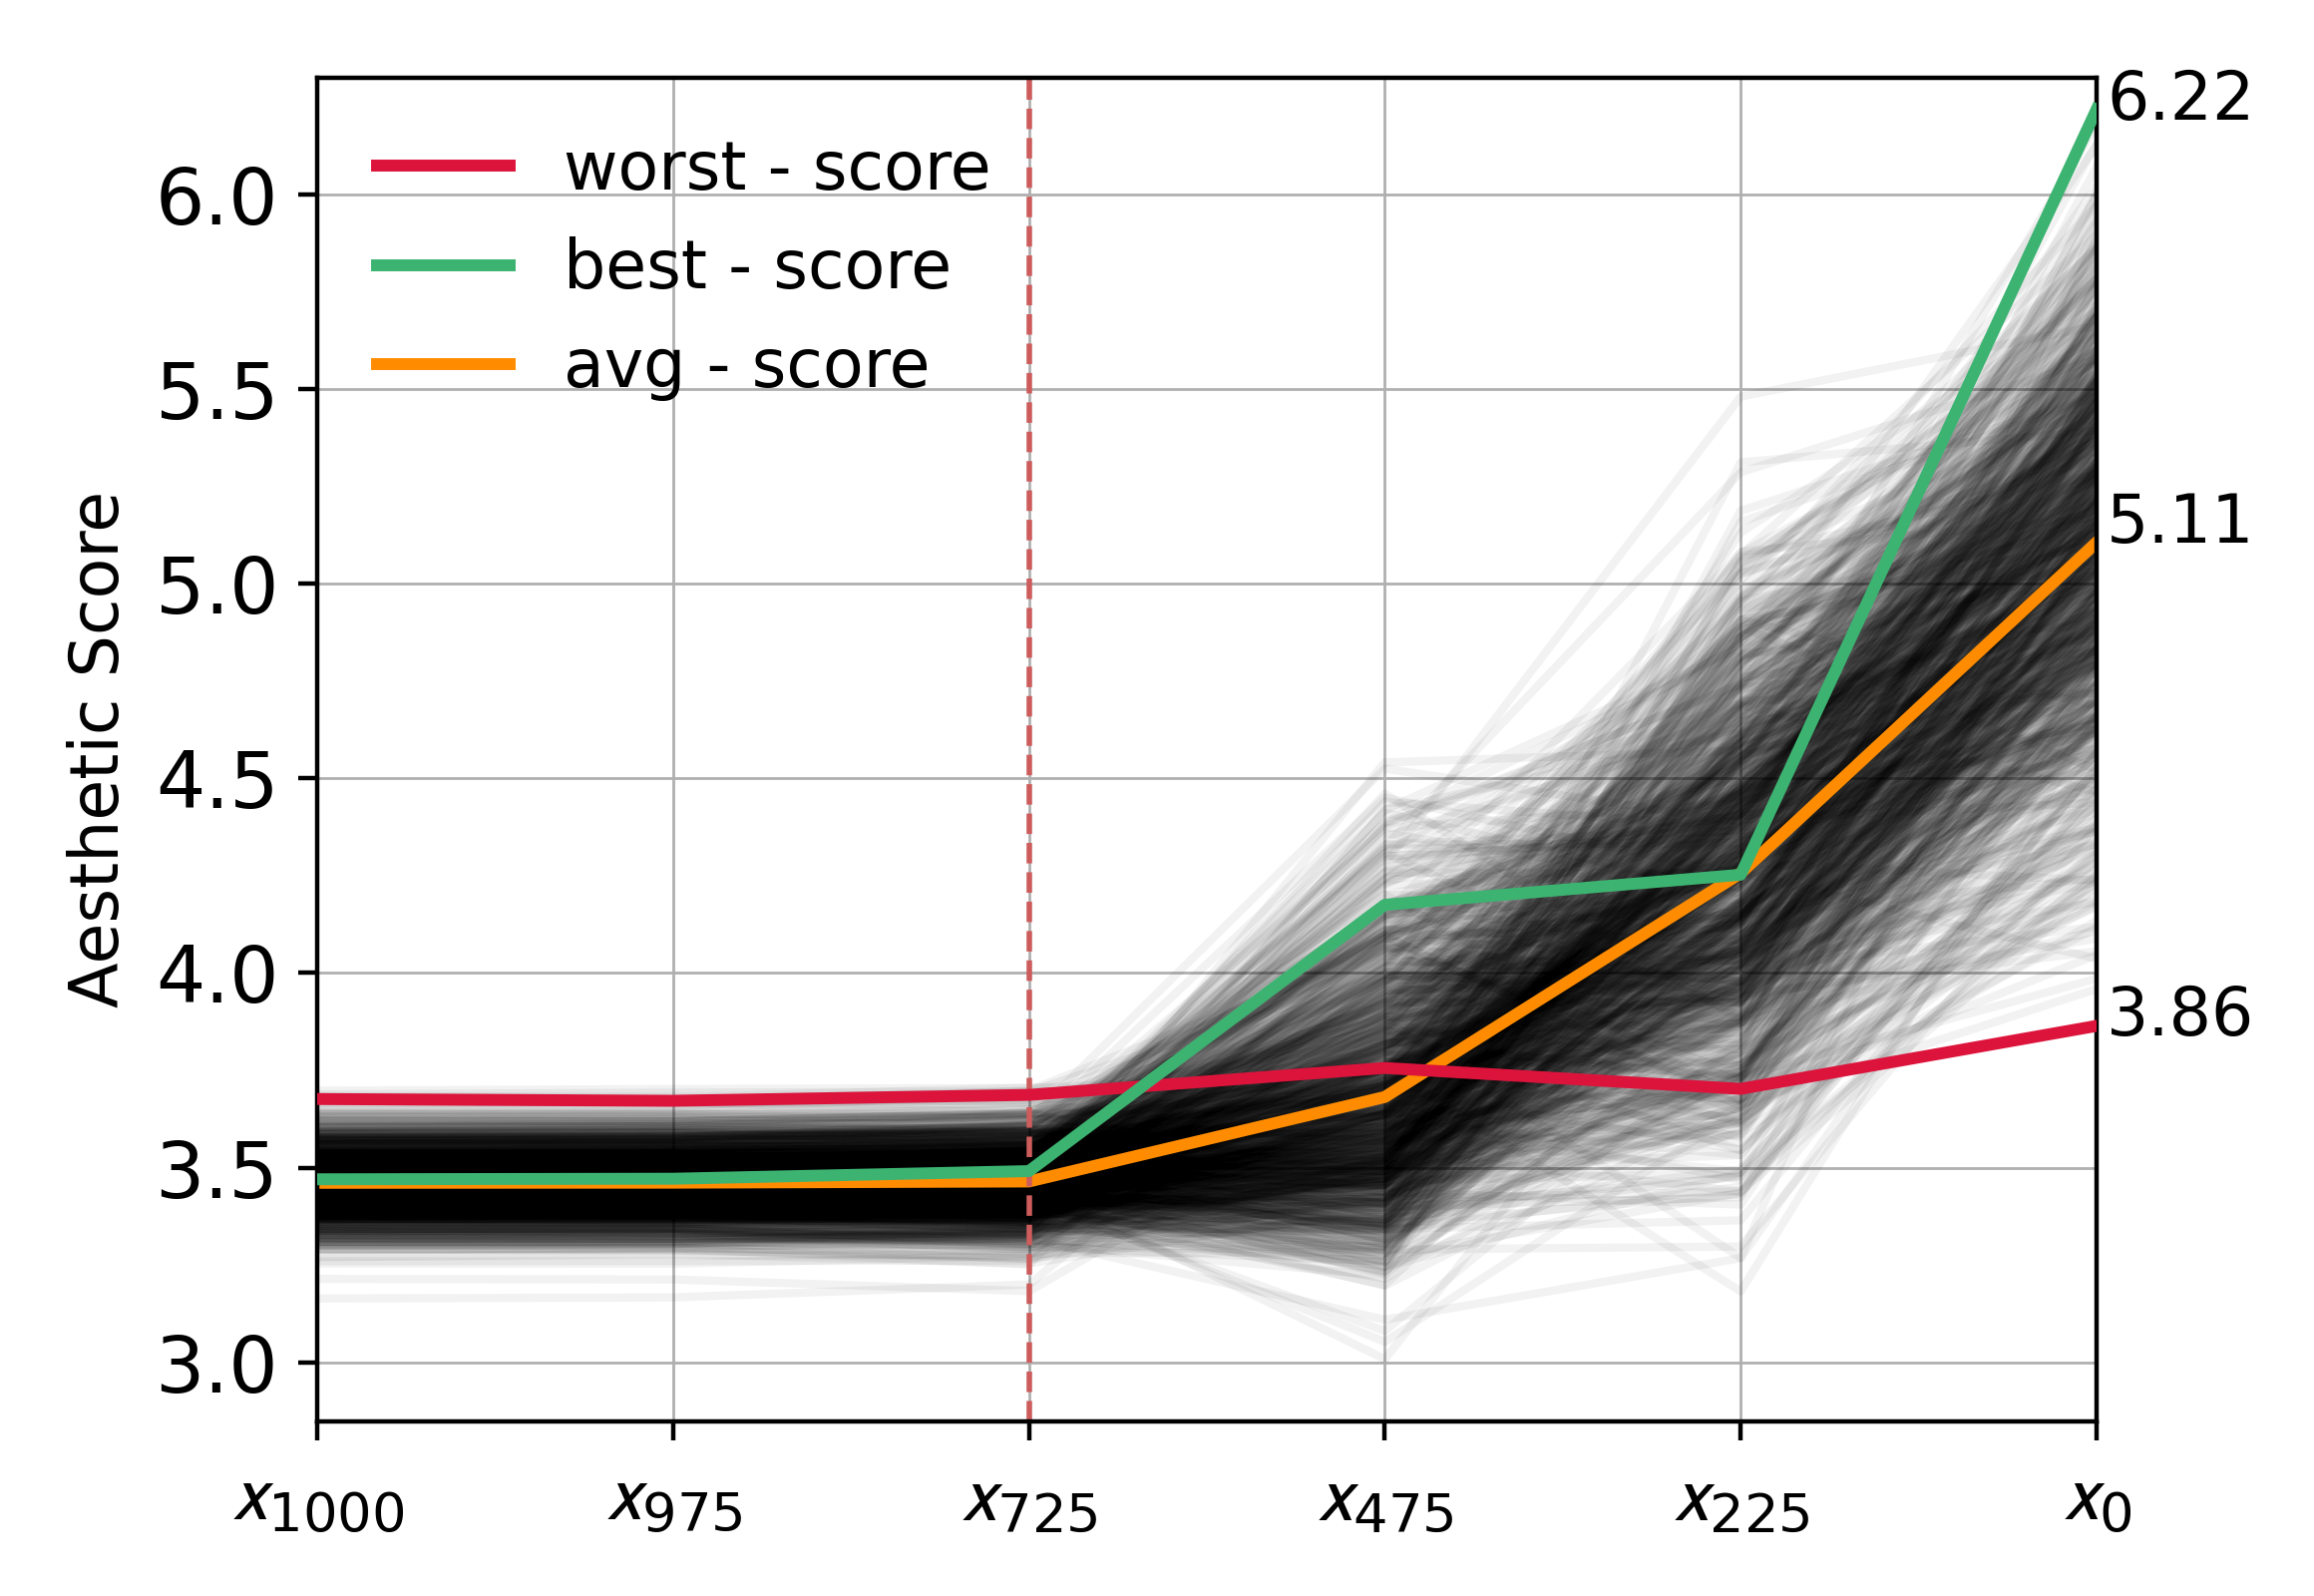
\includegraphics[width=1\textwidth]{img/results/1k-trajectories-aestheic-score-single.png} % first figure itself
  \end{minipage}\hfill
  \begin{minipage}{0.5\textwidth}
      \centering
      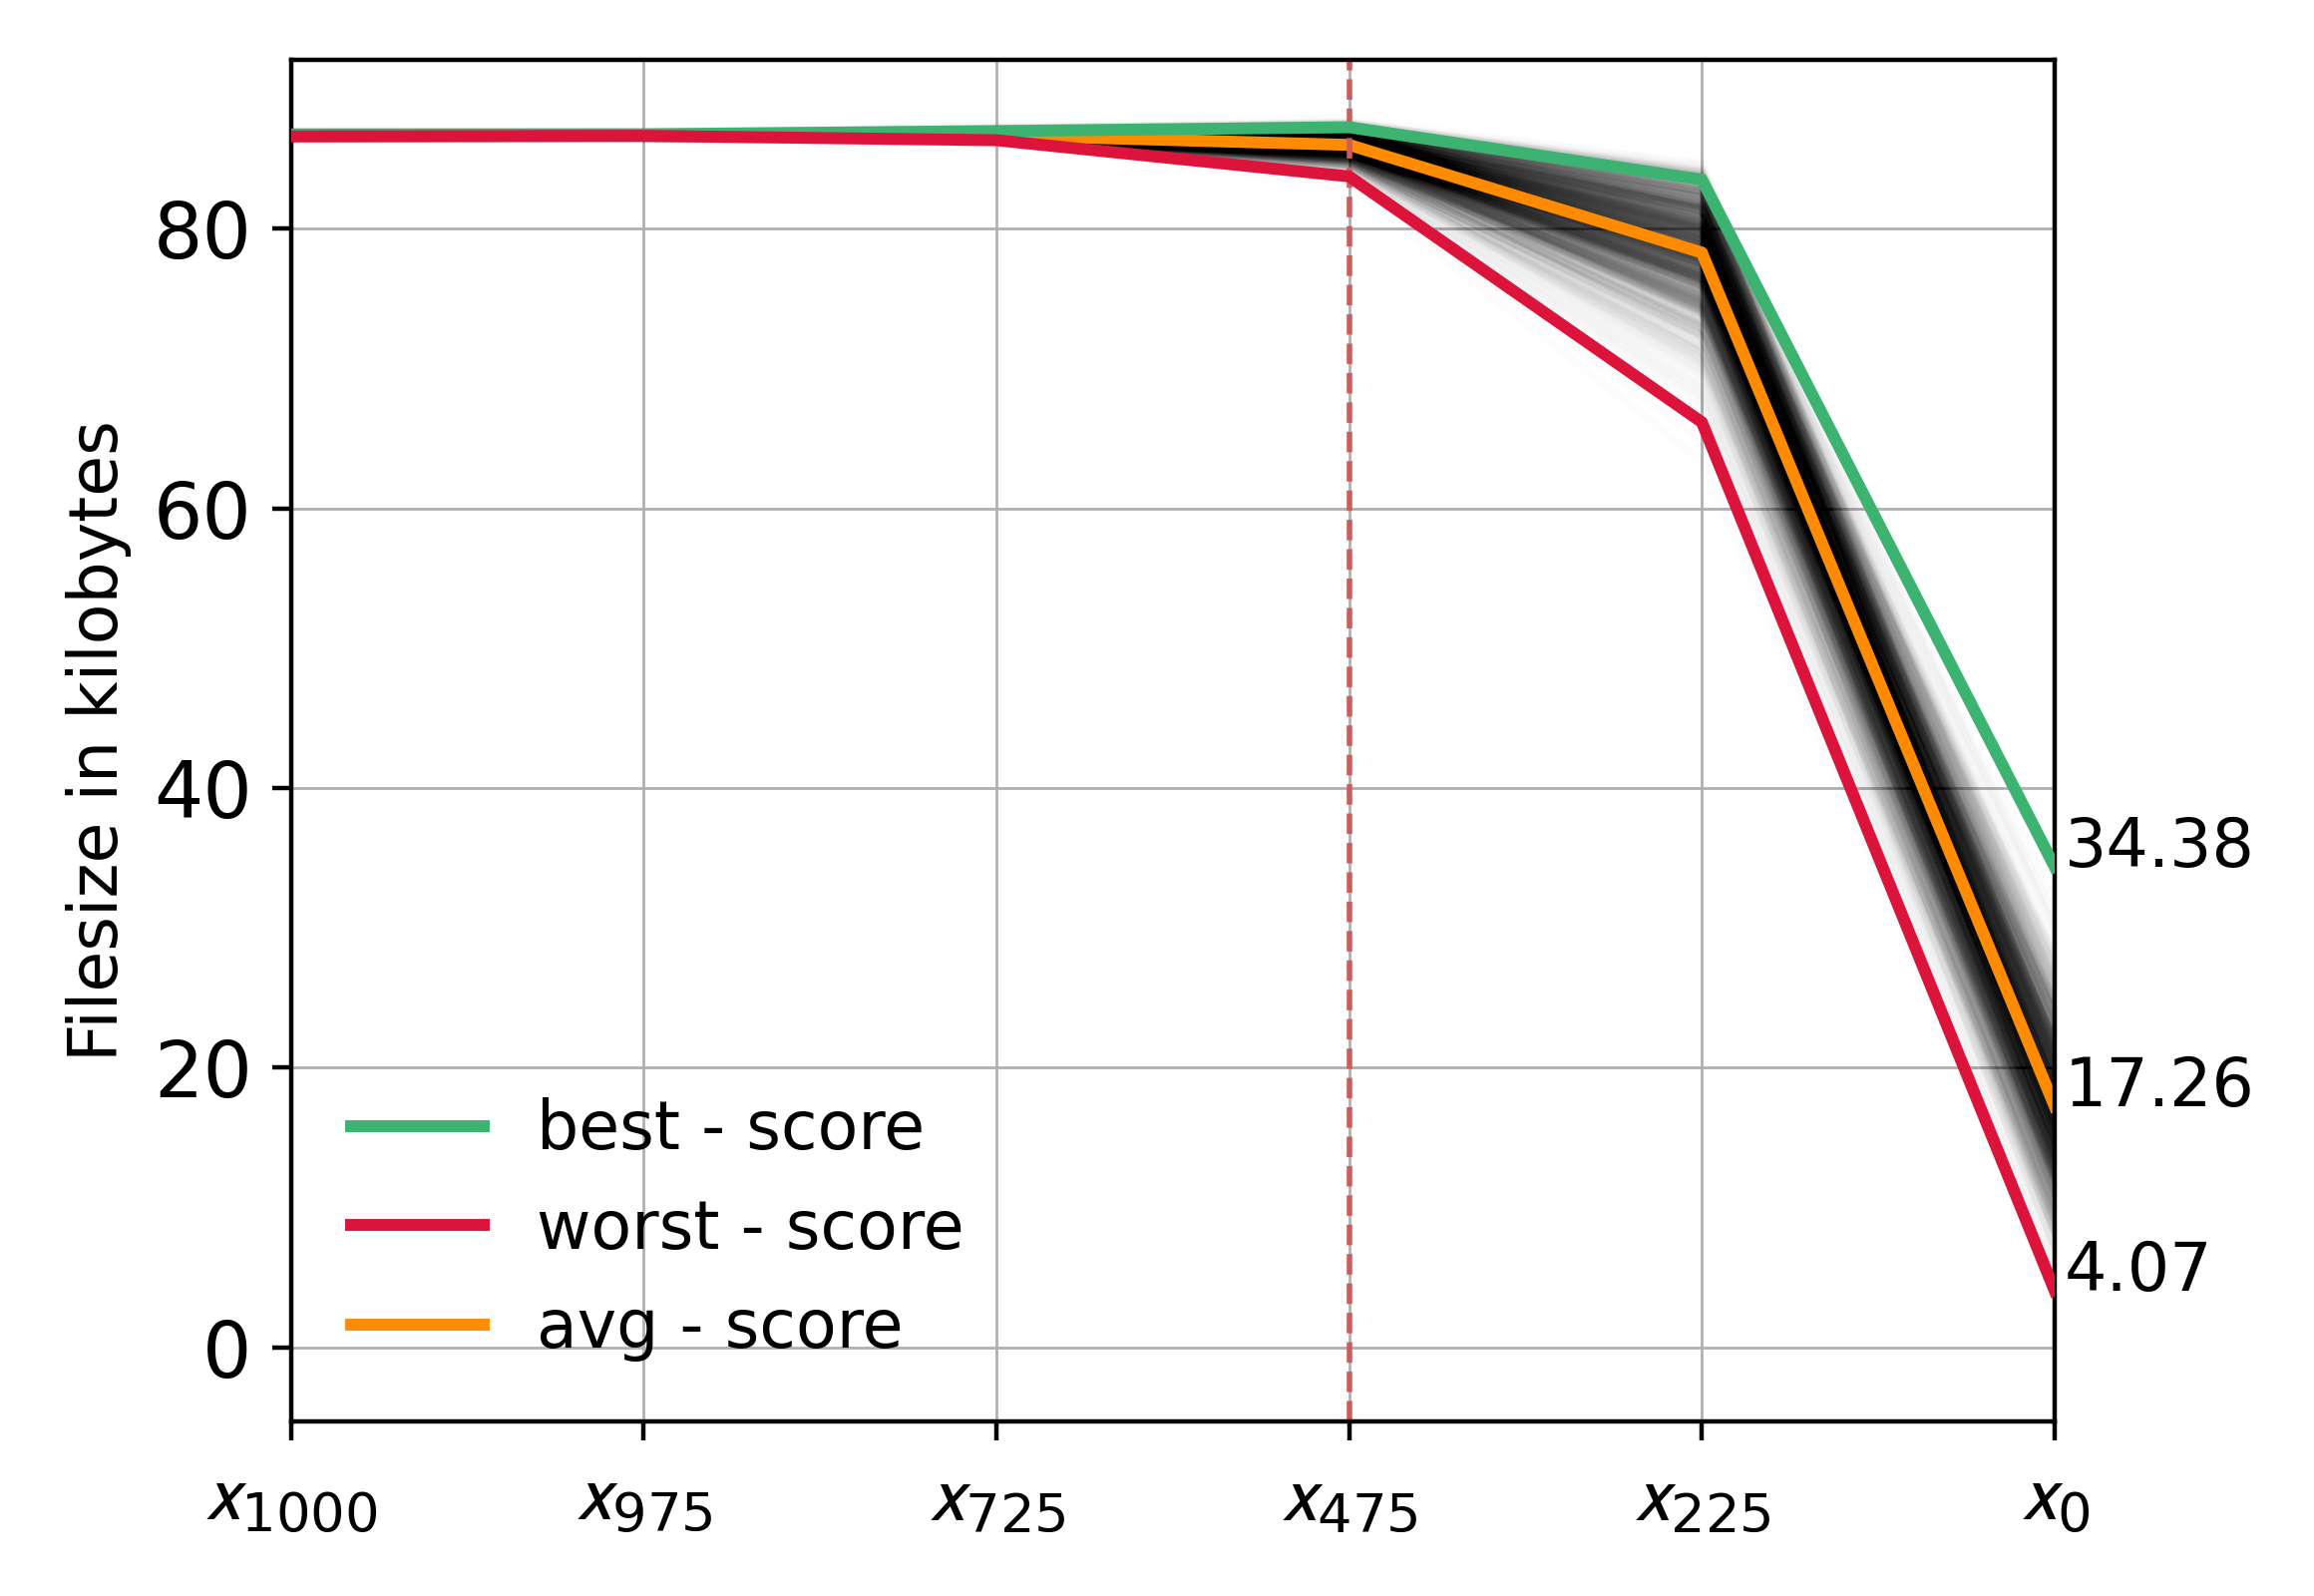
\includegraphics[width=1\textwidth]{img/results/1k-trajectories-jpeg-size-single.png} % second figure itself
  \end{minipage}\vspace{-0.1cm} % space between row 1 and row 2 of figures
  \begin{minipage}{0.5\textwidth}
      \centering
      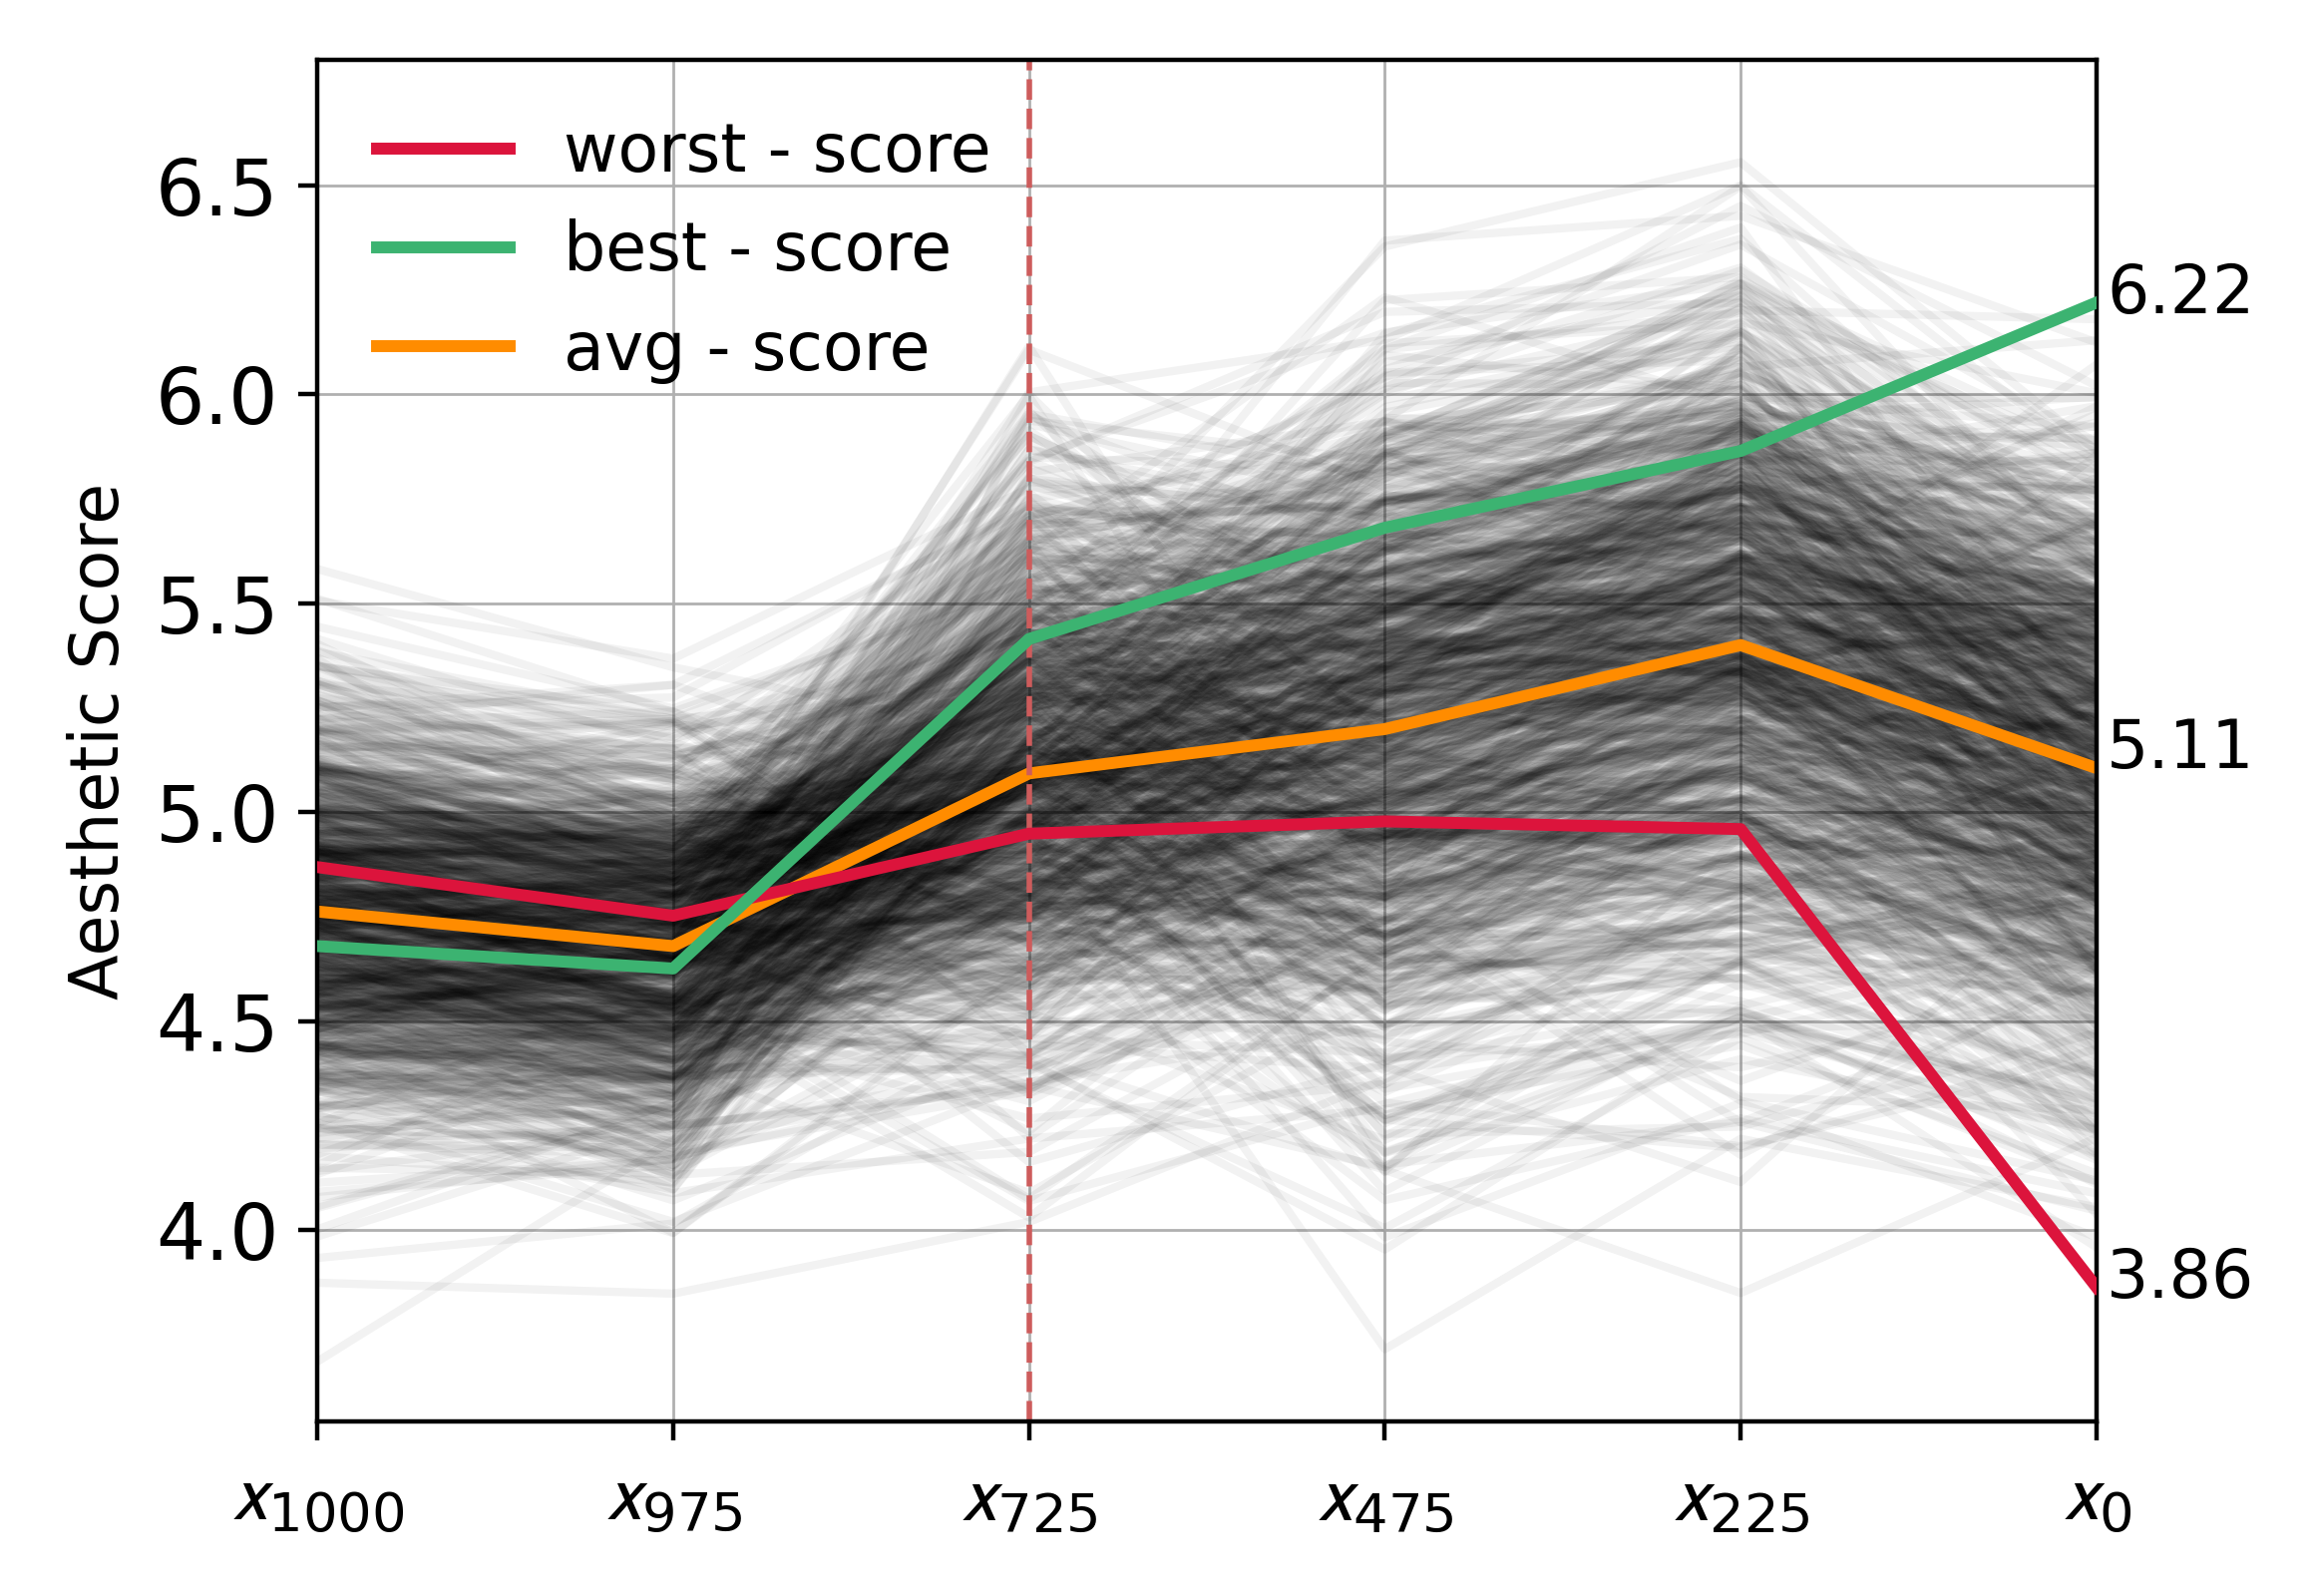
\includegraphics[width=1\textwidth]{img/results/1k-denoise-trajectories-aestheic-score-single.png} % first figure itself
  \end{minipage}\hfill
  \begin{minipage}{0.5\textwidth}
      \centering
      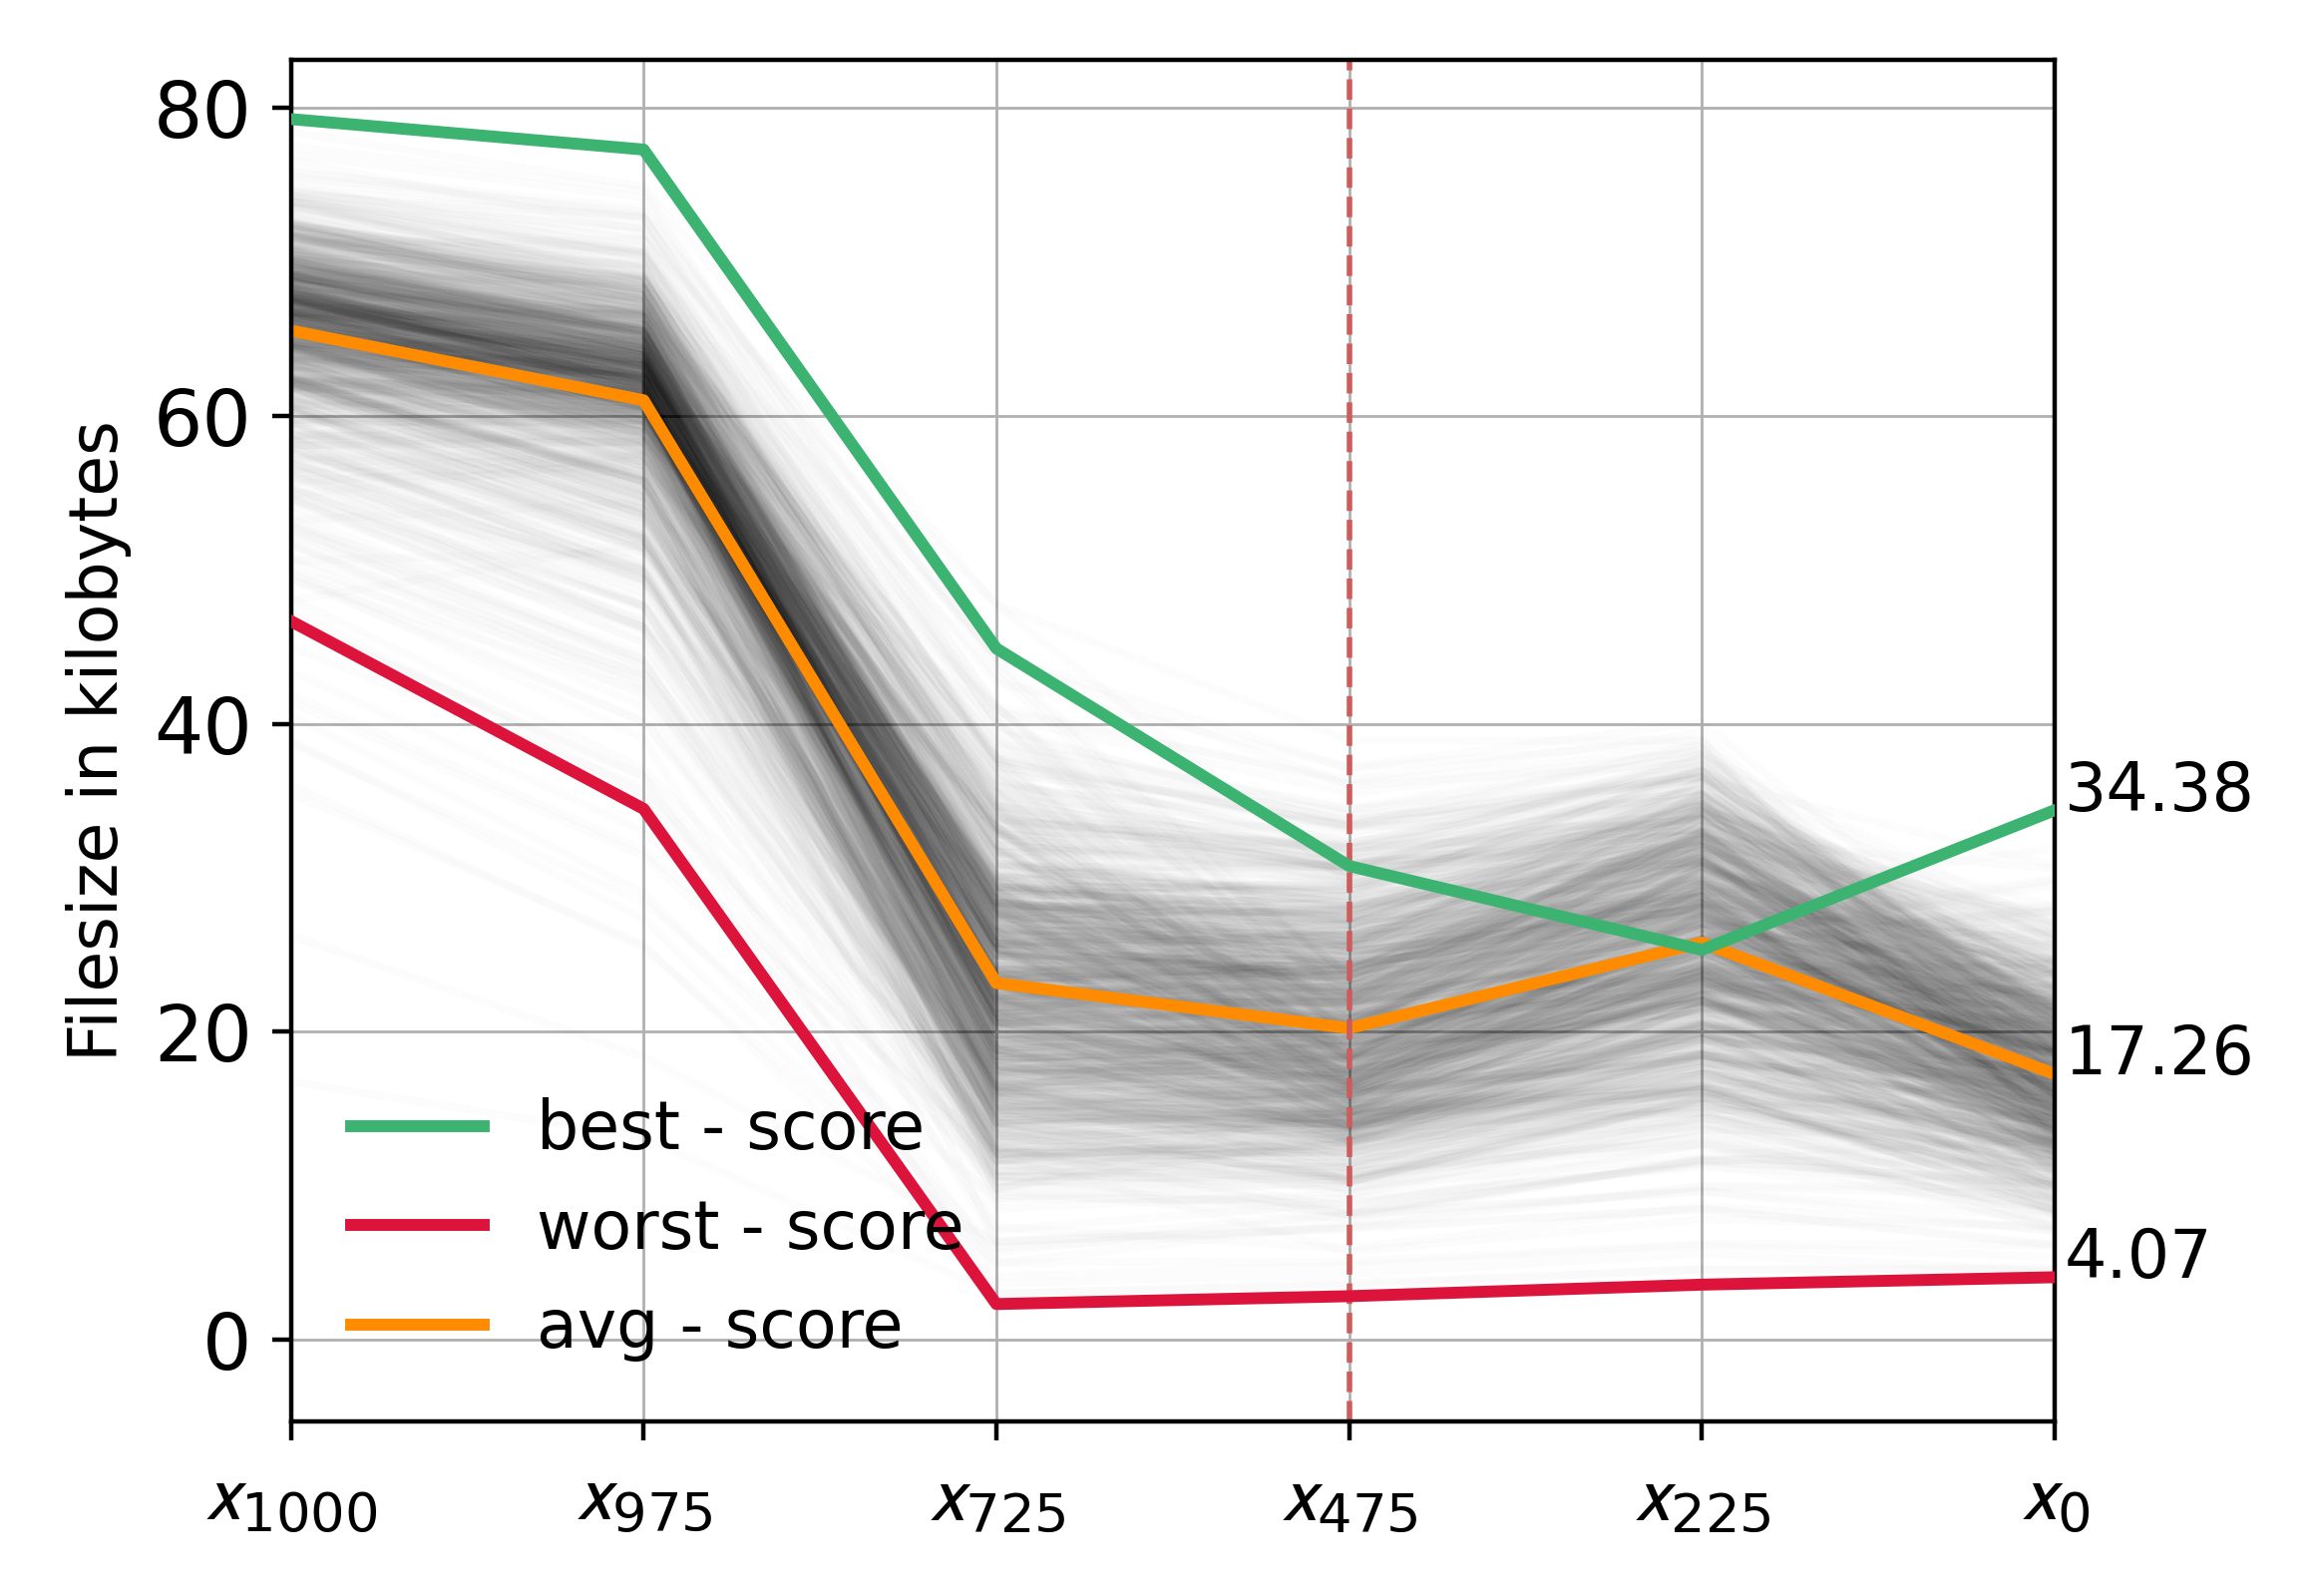
\includegraphics[width=1\textwidth]{img/results/1k-denoise-trajectories-jpeg-size-single.png} % second figure itself
  \end{minipage}
  \vspace{-8pt}  % reduce space between caption and figure
    \captionsetup{width=\textwidth} % set the width of the caption
    \caption{\textbf{Visualizing reward signal during sample trajectories.} \textbf{Left:} Evolution of the aesthetic quality as reward signal over the six states $\mathrm{x}_{\tilde{t}}$, summarizing each of the $1000$ trajectories. \textbf{Right:} Image size in kbs after JPEG compression, providing another form of reward signal for the same set of trajectories. \textbf{Top:} Rewards computed over the noisy intermediate states $\mathrm{x}_{\tilde{t}}$. \textbf{Bottom:} Rewards computed over the denoised states $\tilde{\mathrm{x}}_{\tilde{t}}$.}
  \label{fig:samples-trajectory-rewards} % Add a proper reference for the label
\end{figure}

% \section{Empirical Analysis of Reward Trajectory Dynamics: Insights from DDPM samples}\label{sec:empirical-analysis}

\section{Empirical Analysis on Reward Trajectory Dynamics}\label{sec:empirical-analysis}

% 1er párrafo sección de análisis empírico
\textbf{Is the reward behavior informative during sample trajectories?} The previous discussion about the roadmap to extend the DDPO formulation for using the reward signal from intermediate diffusion states imply that the reward signal is informative throughout the trajectory. This is a key aspect to consider when applying the reward function in the diffusion model context, as it should guide the agent to maximize the reward. In this section, we present an empirical analysis of the reward signal dynamics during the sample generation process. We leverage the unconditional \href{https://huggingface.co/google/ddpm-celebahq-256}{\texttt{google/ddpm-celebahq-256}} \cite{ho2020denoising} pretrained diffusion model on the celebrities faces dataset (Celebahq-256 \citep{karras2017progressive}) to compile a set of trajectory samples, denoted as $\mathcal{S}_o$. \\

\noindent The $1000$ observations in $\mathcal{S}_{0}$ comprises a summary of six intermediate states extracted from each trajectory. We will sample from the model using a $40$ step subsequence $\tau$ of the diffusion chain using the \texttt{DDIMScheduler} \cite{song2020denoising}, speeding up the sampling process over the original diffusion chain of $T=1000$ steps, as we explained in section~\ref{sec:DDIM}. For computational constraint, only six intermediate state of the subsequence $\tau$ are saved, and the equivalence of this summary states $\mathrm{x}_{\tilde{t}}$ with the original DDPM steps are given in the following tuples: $(\tilde{t}=0, t=1000), (\tilde{t}=1, t=975), (\tilde{t}=2, t=725), (\tilde{t}=3, t=475), (\tilde{t}=4, t=225), (\tilde{t}=5, t=0)$. Therefore,
the trajectories are describe starting from the Gaussian noise, then jumping to the step $975$, $725$, until the final sample $\mathrm{x}_{t=0}$, or $\mathrm{x}_{\tilde{t}=5}$. \\

%The reward signal for each state is obtained using the LAION aesthetic predictor and the image size after JPEG compression. The results are shown in Figure~\ref{fig:samples-trajectory-rewards}. \\

\noindent The analysis include two different reward functions. The first one is the LAION aesthetic predictor \cite{laion2022}, a multilayer perceptron (MLP) that assigns a scalar value from 1 to 10 to indicate the aesthetic quality of an image, and it was trained based on human preferences. The second reward function is the image size after JPEG compression algorithm, which is used to define two downstream tasks: compressibility and incompressibility. For compressibility, we want to maximize the negative size of the image after compression, which is equivalent to minimizing the size of the image after compression. The opposite is to maximize the size of the image after compression, which we refer to as incompressibility \ca{Quizás en esta parte solo presentar las funciones de reward y dejar lo de maximizar y minimzar el JPEG compression para la sección de experimentos...}. The election of these reward functions were based to match the experimental pipeline use in the work that introduces DDPO \cite{black2023training}. \\

\noindent Computing the reward over each trajectory on $\mathcal{S}_{0}$ allows us to inspect the reward behavior over the sample trajectories, as shown in the top row of Figure~\ref{fig:samples-trajectory-rewards}. For the aesthetic quality (left), it is possible to observe that from the step $t=725$ ahead, the reward signal start to increase in average (orange line) and a higher variance in the reward signal is observe as the trajectory approach to the final sample $\mathrm{x}_{0}$. During approximately the first $25\%$ of the denoising process, the signal is concentrate with minor variation between a $3.5$ aesthetic score. That is close to the aesthetic score that we obtain when we apply the LAION aesthetic predictor to a purely gaussian random noise. At the end, we achieve a $5.11$ average (orange line) aesthetic score, a $6.22$ and $3.86$ corresponding to the best (green line) and worst (red line) aesthetic score. \\

\noindent For the image size after JPEG compression (right), the reward signal is more stable over the trajectory, and the variance is lower than the aesthetic quality reward signal. The average image size of the final samples after JPEG compression is $17.26$ kilobytes (orange line), and the best (green line) and worst (red line) filesizes are $34.38$ and $4.07$ kilobytes, respectively. The results show that the reward signal start to be some informative on intermediate states from the step $t=475$ ahead, but with a lower variance than the aesthetic quality reward signal. The reason is that the noise is difficult to compress, and the JPEG compression can start to have effects on the image size reduction when the semantic of the image start to appear and the entropy is reduce.  \\

\noindent The top row of Figure~\ref{fig:samples-trajectory-rewards} shows the rewards computed directly over the intermediate states, i.e. structure plus noise. However, there is an issue in doing this, and could be the reason of why is a good idea to only compute the reward on the final samples $\mathrm{x}_{0}$, as is illustated in the Markov
Decision Process (MDP) formulation for a diffusion a model in Figure~\ref{fig:diffusion-model-mdp}. The reward function to control the model is design to maximize the reward in the final sample, which is a state that can be directly guide by the human preferences. Of course that we can 
provide human preferences between noisy states, but nothing guarantee that
the denoising trajectories will be consistent in the following states. Similar with the JPEG compression, the goal is to generate images of lower size, and
this endeavour it has nothing to do with the noise involved in the sample generation process. Therefore, we have a communicational gap between the intermediate states and the reward signal, a similar problem that occur using
classifier guidance with a model that is not robust to the noise to guide
the generative process \cite{bansal2023universal}. \\

\noindent \noindent \textbf{Denoised sample trajectories.} We will use the denoised observations $\tilde{\mathrm{x}}_{t\rightarrow 0}$ for the initial
noise and each intermediate step $t$ of the sample trajectories, as referred in the DDIM section~\ref{sec:DDIM}:
\begin{equation}\label{eqn:ddim-predicted-sample}
  \tilde{\mathrm{x}}_{t\rightarrow0}=f_{\theta}^{(t)}=\frac{\mathrm{x}_{t}-\sqrt{1-\alpha_{t}}\epsilon_{\theta}^{(t)}(\mathrm{x}_{t})}{\sqrt{\alpha_{t}}}
\end{equation}

\noindent As you can see in Figure~\ref{fig:sample-trajectories}, the denoised samples $\tilde{\mathrm{x}}_{t\rightarrow0}$ are fairly similar to the
final sample. The denoised intermediate state $\tilde{\mathrm{x}}_{725\rightarrow0}$ almost captures the essence of the final sample $\mathrm{x}_{0}$, and $\tilde{\mathrm{x}}_{1000\rightarrow0}$ is a highly informative latent encode of the high level features such image pose, gender, hair style and colors of the final image. Notice that in the same point in Figure~\ref{fig:samples-trajectory-rewards} (bottom-left), we have an increasing dispersion in the aesthetic score trajectory distribution from the start. This is a clear indication that the reward signal is more informative in the denoised samples than in the noisy samples. The same behavior is observed for the image size after JPEG compression (bottom-right), where the variance is higher in the denoised samples than in the noisy samples. That is because the
JPEG compressioon knows in advance which trajectories contain features that can be compressed or not.

% Trayectorias resumidas de google/ddpm-celebahq-256 usando DDIM scheduler y con
% los estados intermedios denoised usando formula DDIM. Se reportan los reward
% de cada imagen...
\begin{figure}[ht]
  \centering
  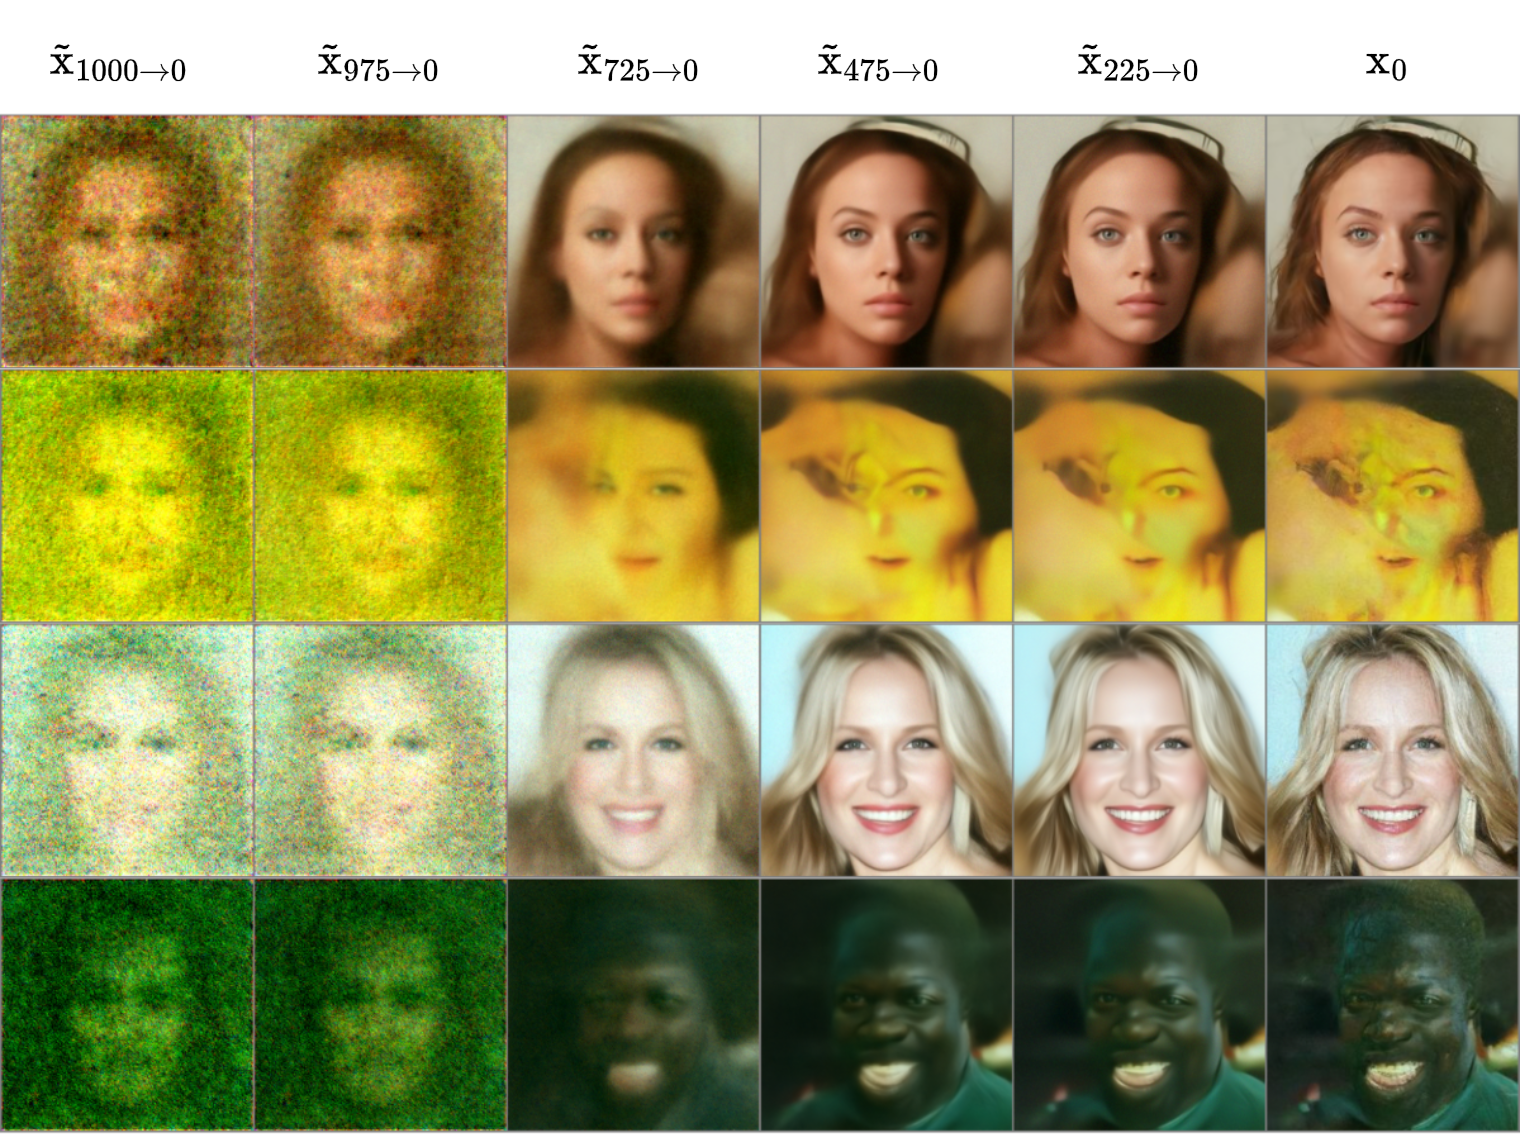
\includegraphics[scale=0.85]{img/results/denoised-samples-trajectories.png}
  \vspace{-5pt}  % reduce space between caption and figure
    \captionsetup{width=\textwidth} % set the width of the caption
    \caption{\textbf{Denoised sample trajectories.} Each row, from \textbf{top-to-bottom}, represents the best ($6.22$)
  and worst ($3.86$) aesthetic scores, and the highest ($34.38$) and lowest 
  ($4.07$) filesizes in kilobytes after JPEG compression for the final samples
  $\mathrm{x}_{0}$ in $\mathcal{S}_{o}$. Each column, from \textbf{left-to-right}, summarizes the states for each denoised sample's trajectory using Eq.~\ref{eqn:ddim-predicted-sample}. The rows correspond to the trajectories highlighted in the green and red lines of Figure~\ref{fig:samples-trajectory-rewards}.}
   \label{fig:sample-trajectories}
\end{figure}


\section{Experiments}

En primer lugar queremos reproducir la implementación propuesta en \textit{Training Diffusion Models with Reinforcement Learning} \cite{black2023training} en un \textit{setting} más simplificado para facilitar
la experimentación, pero que aún capture la complejidad de los text-to-image models para experimentar con \textit{reward functions}. Utilizaremos como \textit{baseline} las capacidades generativas del modelo preentrenado \texttt{google/ddpm-celebahq-256} descrito en \cite{ho2020denoising}. Este es un modelo no condicionado que genera imágenes RGB de 256x256 con rostros de personas. Es un modelo previo a los modelos latentes de difusión, por lo que el proceso de \textit{denoising} ocurre en el espacio de los pixeles. \\

% Se habla sobre la metodología usada para evaluar...
\noindent \textbf{Evaluation dataset.} We use the final samples of each trajectory in $\mathcal{S}_{0}$---\textit{described in the previous section \ref{sec:empirical-analysis}}---as a baseline of the generative capacities of the pretrained model performance on the downstream tasks\footnote{Whenever it refers to DDPM in the context of results, it means that we are measuring the capacities of the pretrained model \texttt{gooogle/ddpm-celebahq-256} with the samples in $\mathcal{S}_{0}$, as referred in Section~\ref{sec:empirical-analysis}.}. In the following sections, the experiments were evaluated using the same seeds to generate the samples but with the finetuned checkpoints, and report the mean and standard error of the rewards over the evaluation samples. This metrics are the quantitative evaluation used in this work to compare the performance of the finetuned models against the pretrained one. \\

\subsection{Reproducing DDPO}

\noindent In our experiments, we employed three downstream tasks as outlined in \cite{black2023training}: compressibility, incompressibility, and aesthetic quality. The first two tasks are defined by the size of images after applying a JPEG compression algorithm, serving as the reward function. For aesthetic quality, we utilized the LAION aesthetic model \citep{laion2022}, a multilayer perceptron that assigns a scalar value from 1 to 10 to indicate the aesthetic quality of an image. \\

\noindent These tasks effectively demonstrate the flexibility of using RL to learn new downstream objectives. Supervised learning finetuning often struggles to encode tasks like compressibility and incompressibility into a loss function, whereas RL can optimize these tasks directly through a reward function. Additionally, the LAION aesthetic model, trained on human preferences, exemplifies how human feedback can be incorporated to align sample generation with desired outcomes. This is a key advantage of using RL with generative models \citep{ouyang2022training}. \\

\noindent Using the size of the image after JPEG compression as reward function, we can define two downstream tasks: \textit{compressibility} and \textit{incompressibility}. For compressibility, we want to maximize the negative size of the image after compression. This is equivalent to minimizing the size of the image after compression. The opposite is to maximize the size of the image after compression, which we refer to as incompressibility. \\

\subsection{Implement I-DDPO}

XYZ

\subsection{Experiment results}
\begin{table}
\centering
\begin{tabular}{lccc}
\toprule
\textbf{Downstream Task} & \textbf{Baseline} & \textbf{DDPO} & \textbf{I-DDPO}\\
\midrule
LAION Aesthetic Score (higher is better) & 5.11 $~\pm$ 0.01 & \textbf{5.58} $~\pm$ 0.01 & - \\
JPEG Compressibility (lower is better) & 17.26 $~\pm$  0.15 & \textbf{6.01} $~\pm$ 0.13  & -\\
JPEG Incompressibility (higher is better) & 17.26 $~\pm$ 0.15 & \textbf{21.6} $~\pm$ 0.12 & - \\
Over 50 years old (higher is better) & -7.72 $~\pm$ 0.17 & \textbf{7.39} $~\pm$ 0.16& - \\
\bottomrule
\end{tabular}
\captionsetup{width=\textwidth} % set the width of the caption
\caption{\textbf{Mean and standard error for rewards associated with each downstream task}. For fairness, all checkpoints used the same initial noise for sample generation. The \textbf{Baseline} refers to the generative capabilities of the pretrained model represented by $\mathcal{S}_{0}$ (Section~\ref{sec:empirical-analysis}). \textbf{DDPO} shows results from a finetuned model using DDPO with importance sampling (Section~\ref{sec:diffusion-model-mdp}). The \textbf{I-DDPO} column represents our proposed method.}
\label{tab:reward-results}
\end{table}

In Table~\ref{tab:reward-results} we have a summary of the results for each downstream tasks. The baseline are the initial performance of the pretrained DDPM model. The results show that the DDPO fintuned models outperform the baseline in all tasks, regarding the mean reward over the evaluation samples. A set of images generated under the same initial noise by the pretrained model and the finetuned models are provided for a quality comparison in Figure~\ref{fig:visual-comparison-ddpo}. In most cases, the general semantic of faces mantain---\textit{still identifying the same subject what
is depicted in the original sample}---while DDPO induce modification at high level features to achieve the reward objective. Additional comparative samples in the Appendix~\ref{appendix:additional-samples}. \\

% \ca{\textbf{TODO:} Mencionar la metodologia de evaluación usando $\mathcal{S}_{0}$ y $\mathcal{S}_{f}$, siendo muestras generadas a partir del mismo ruido
% inicial, pero denoseadas usando el checkpoint $f$ finetuneado con RL en un
% downstream particular. De esta forma, podemos comparar en conjunto de evaluación variaciones en las muestras sin el efecto de puntos de partida distintos.}

% Mean and Reward Histograms for JPEG compressibility and incompressibility
\begin{figure}[ht]
  \centering
  \begin{minipage}{0.5\textwidth}
      \centering
      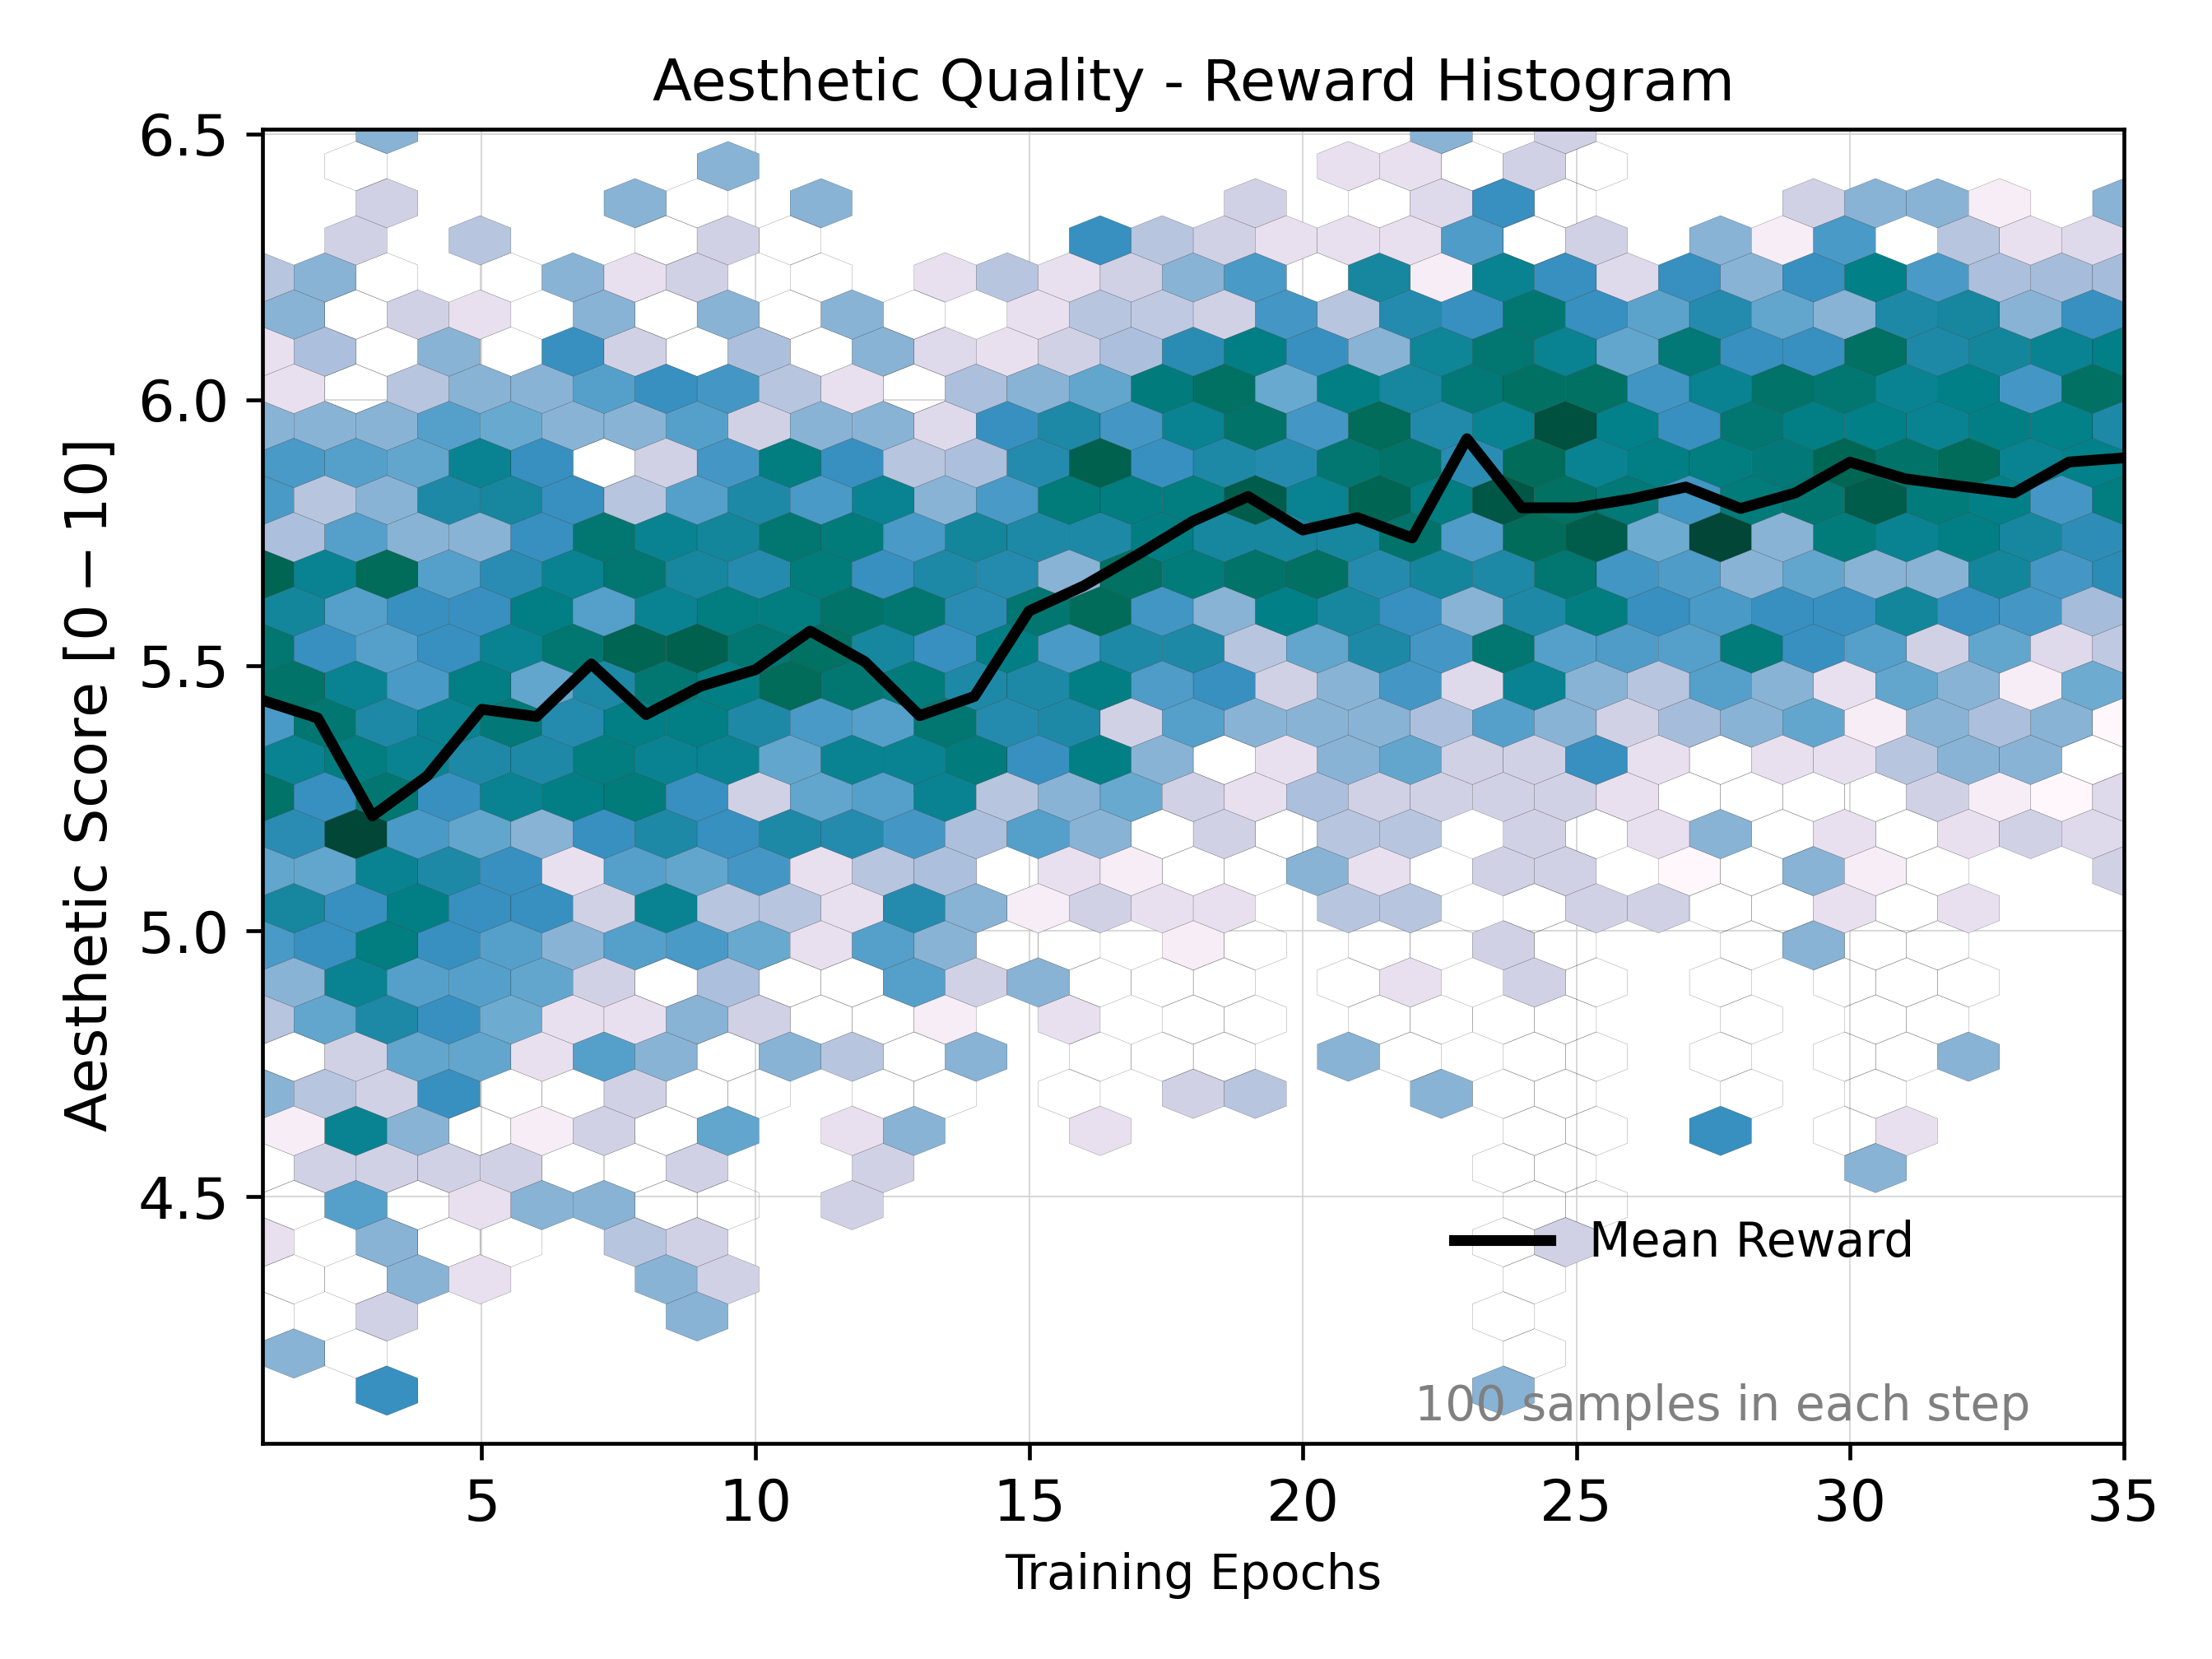
\includegraphics[width=1\textwidth]{img/results/reward_hist-laion-aesthetic.png} % first figure itself
      %\label{fig:sample_figure_1}
  \end{minipage}\hfill
  \begin{minipage}{0.5\textwidth}
      \centering
      % 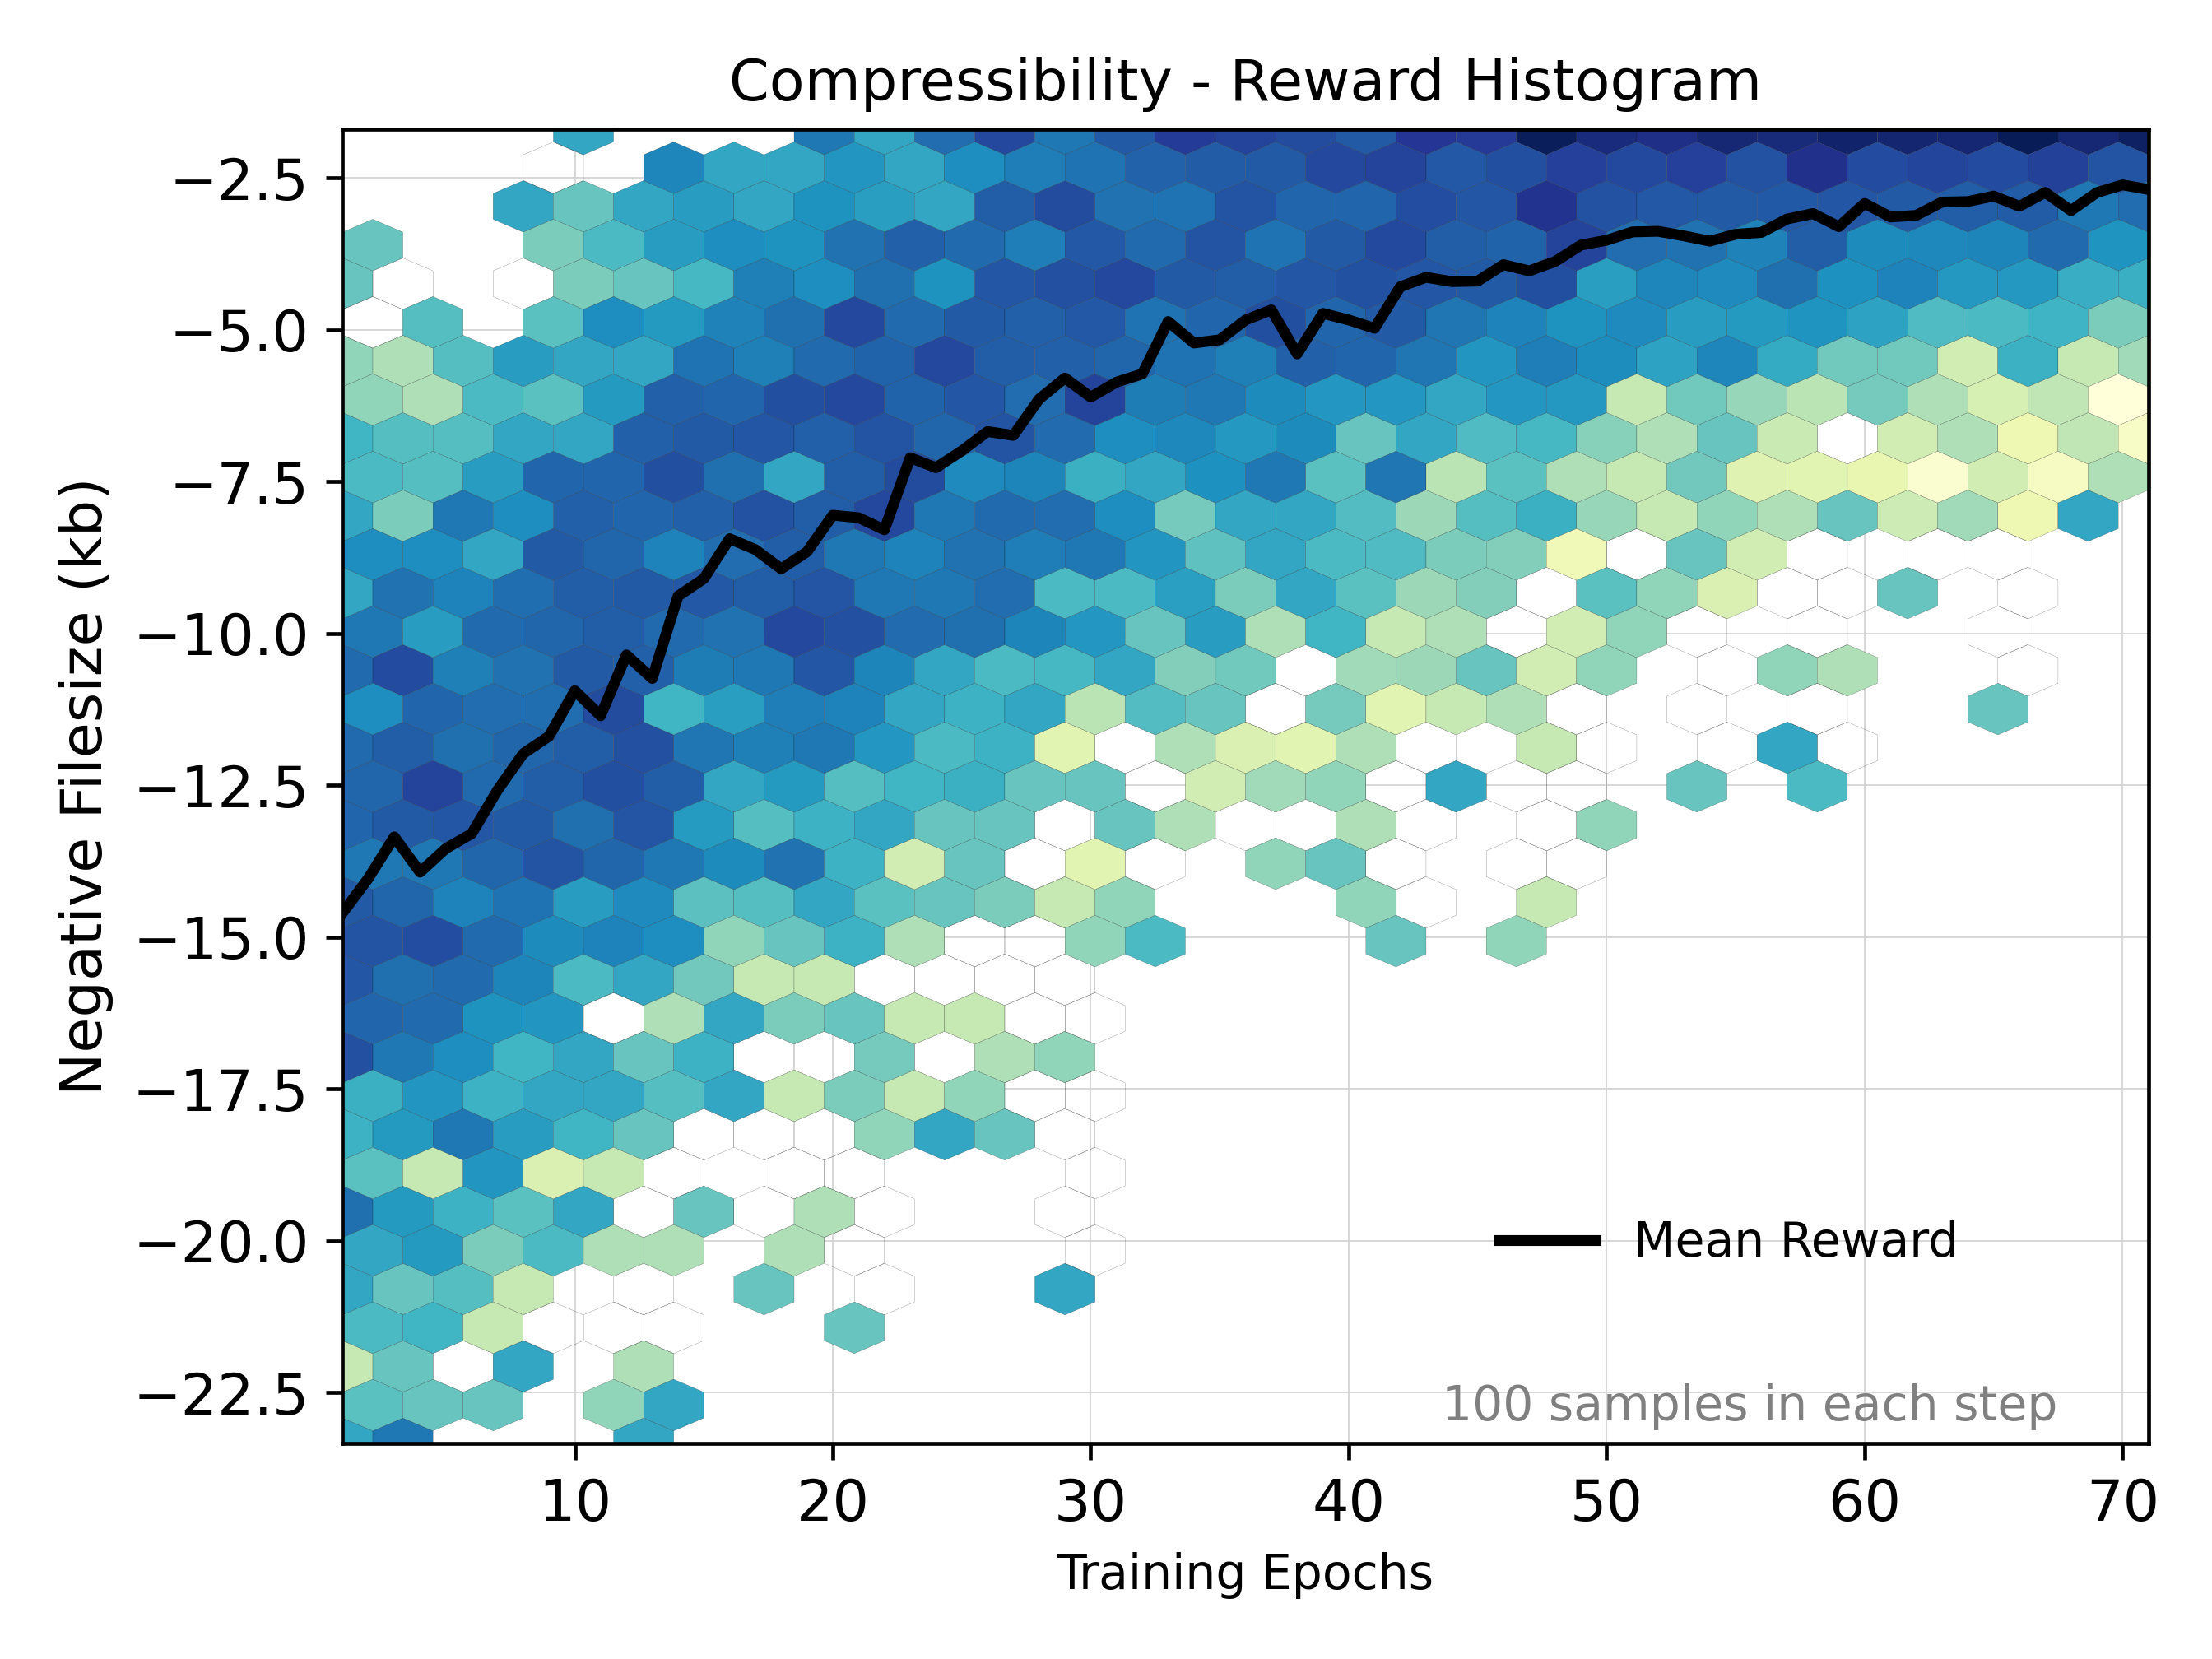
\includegraphics[width=1\textwidth]{img/results/reward_hist-jpeg-compressibility.png} % second figure itself
      %\label{fig:sample_figure_2}
  \end{minipage}\vspace{-0.1cm} % space between row 1 and row 2 of figures
  \begin{minipage}{0.5\textwidth}
      \centering
      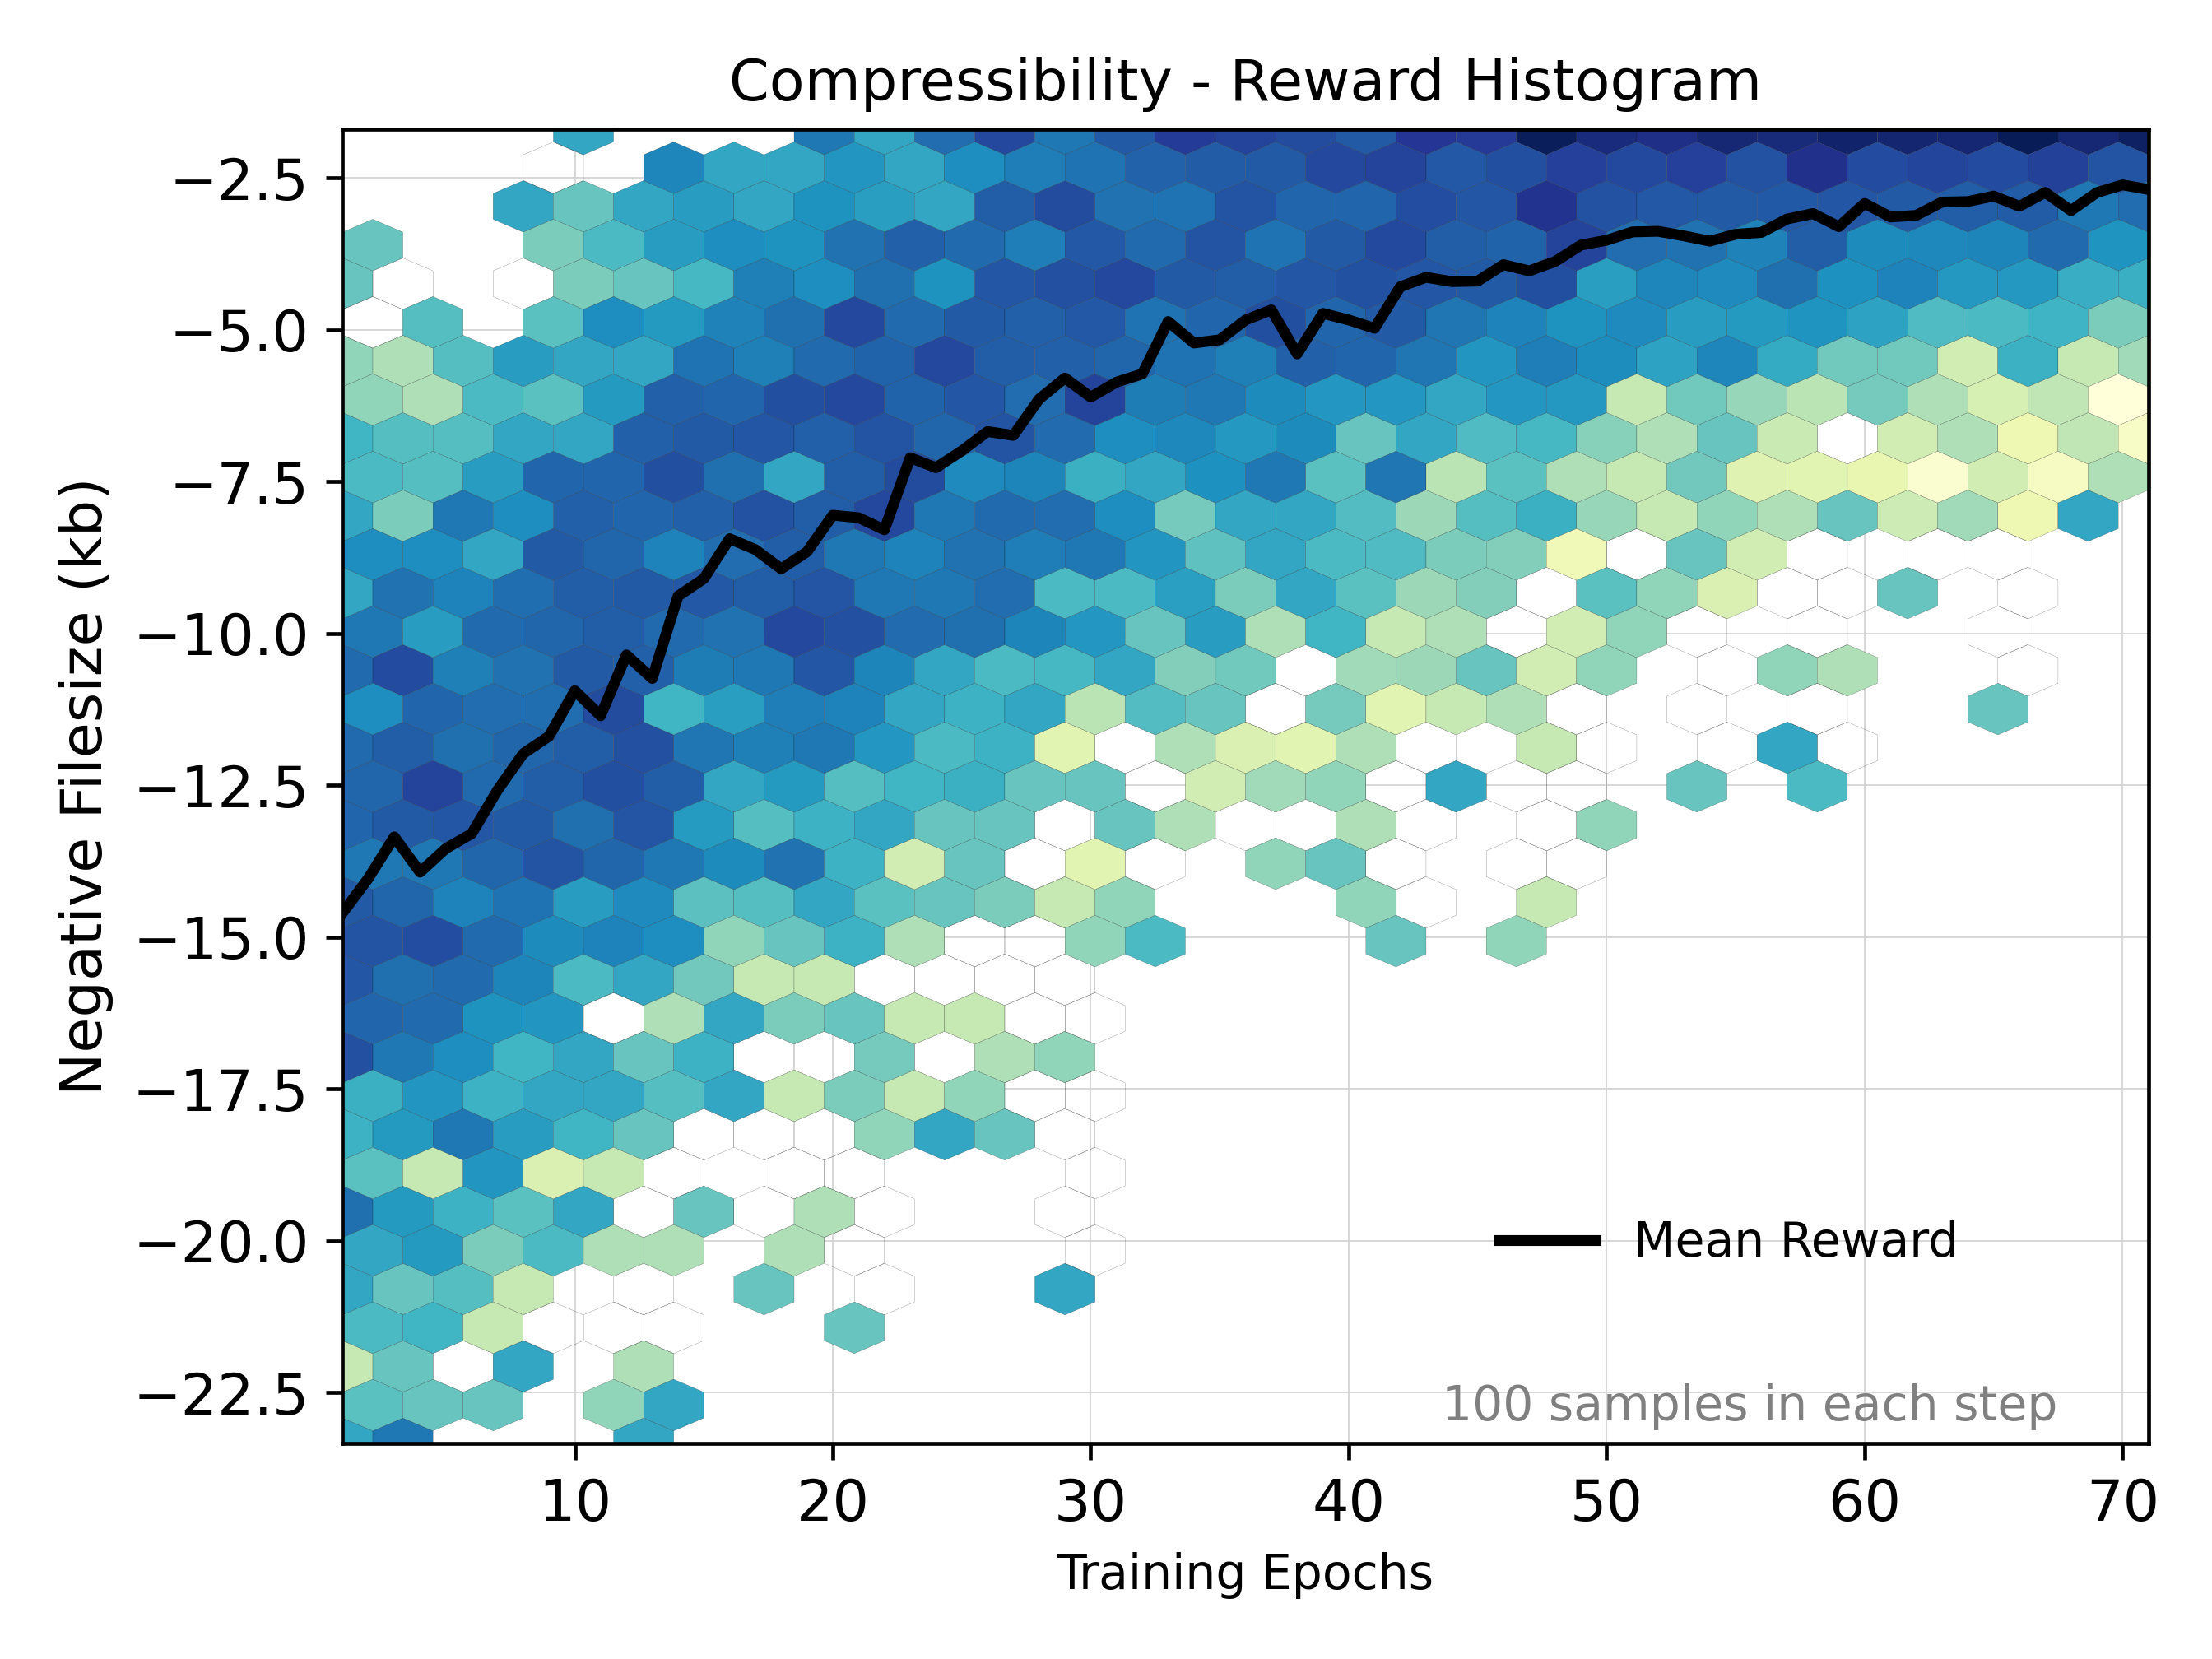
\includegraphics[width=1\textwidth]{img/results/reward_hist-jpeg-compressibility.png} % third figure itself
      %\label{fig:sample_figure_3}
  \end{minipage}\hfill
  \begin{minipage}{0.5\textwidth}
      \centering
      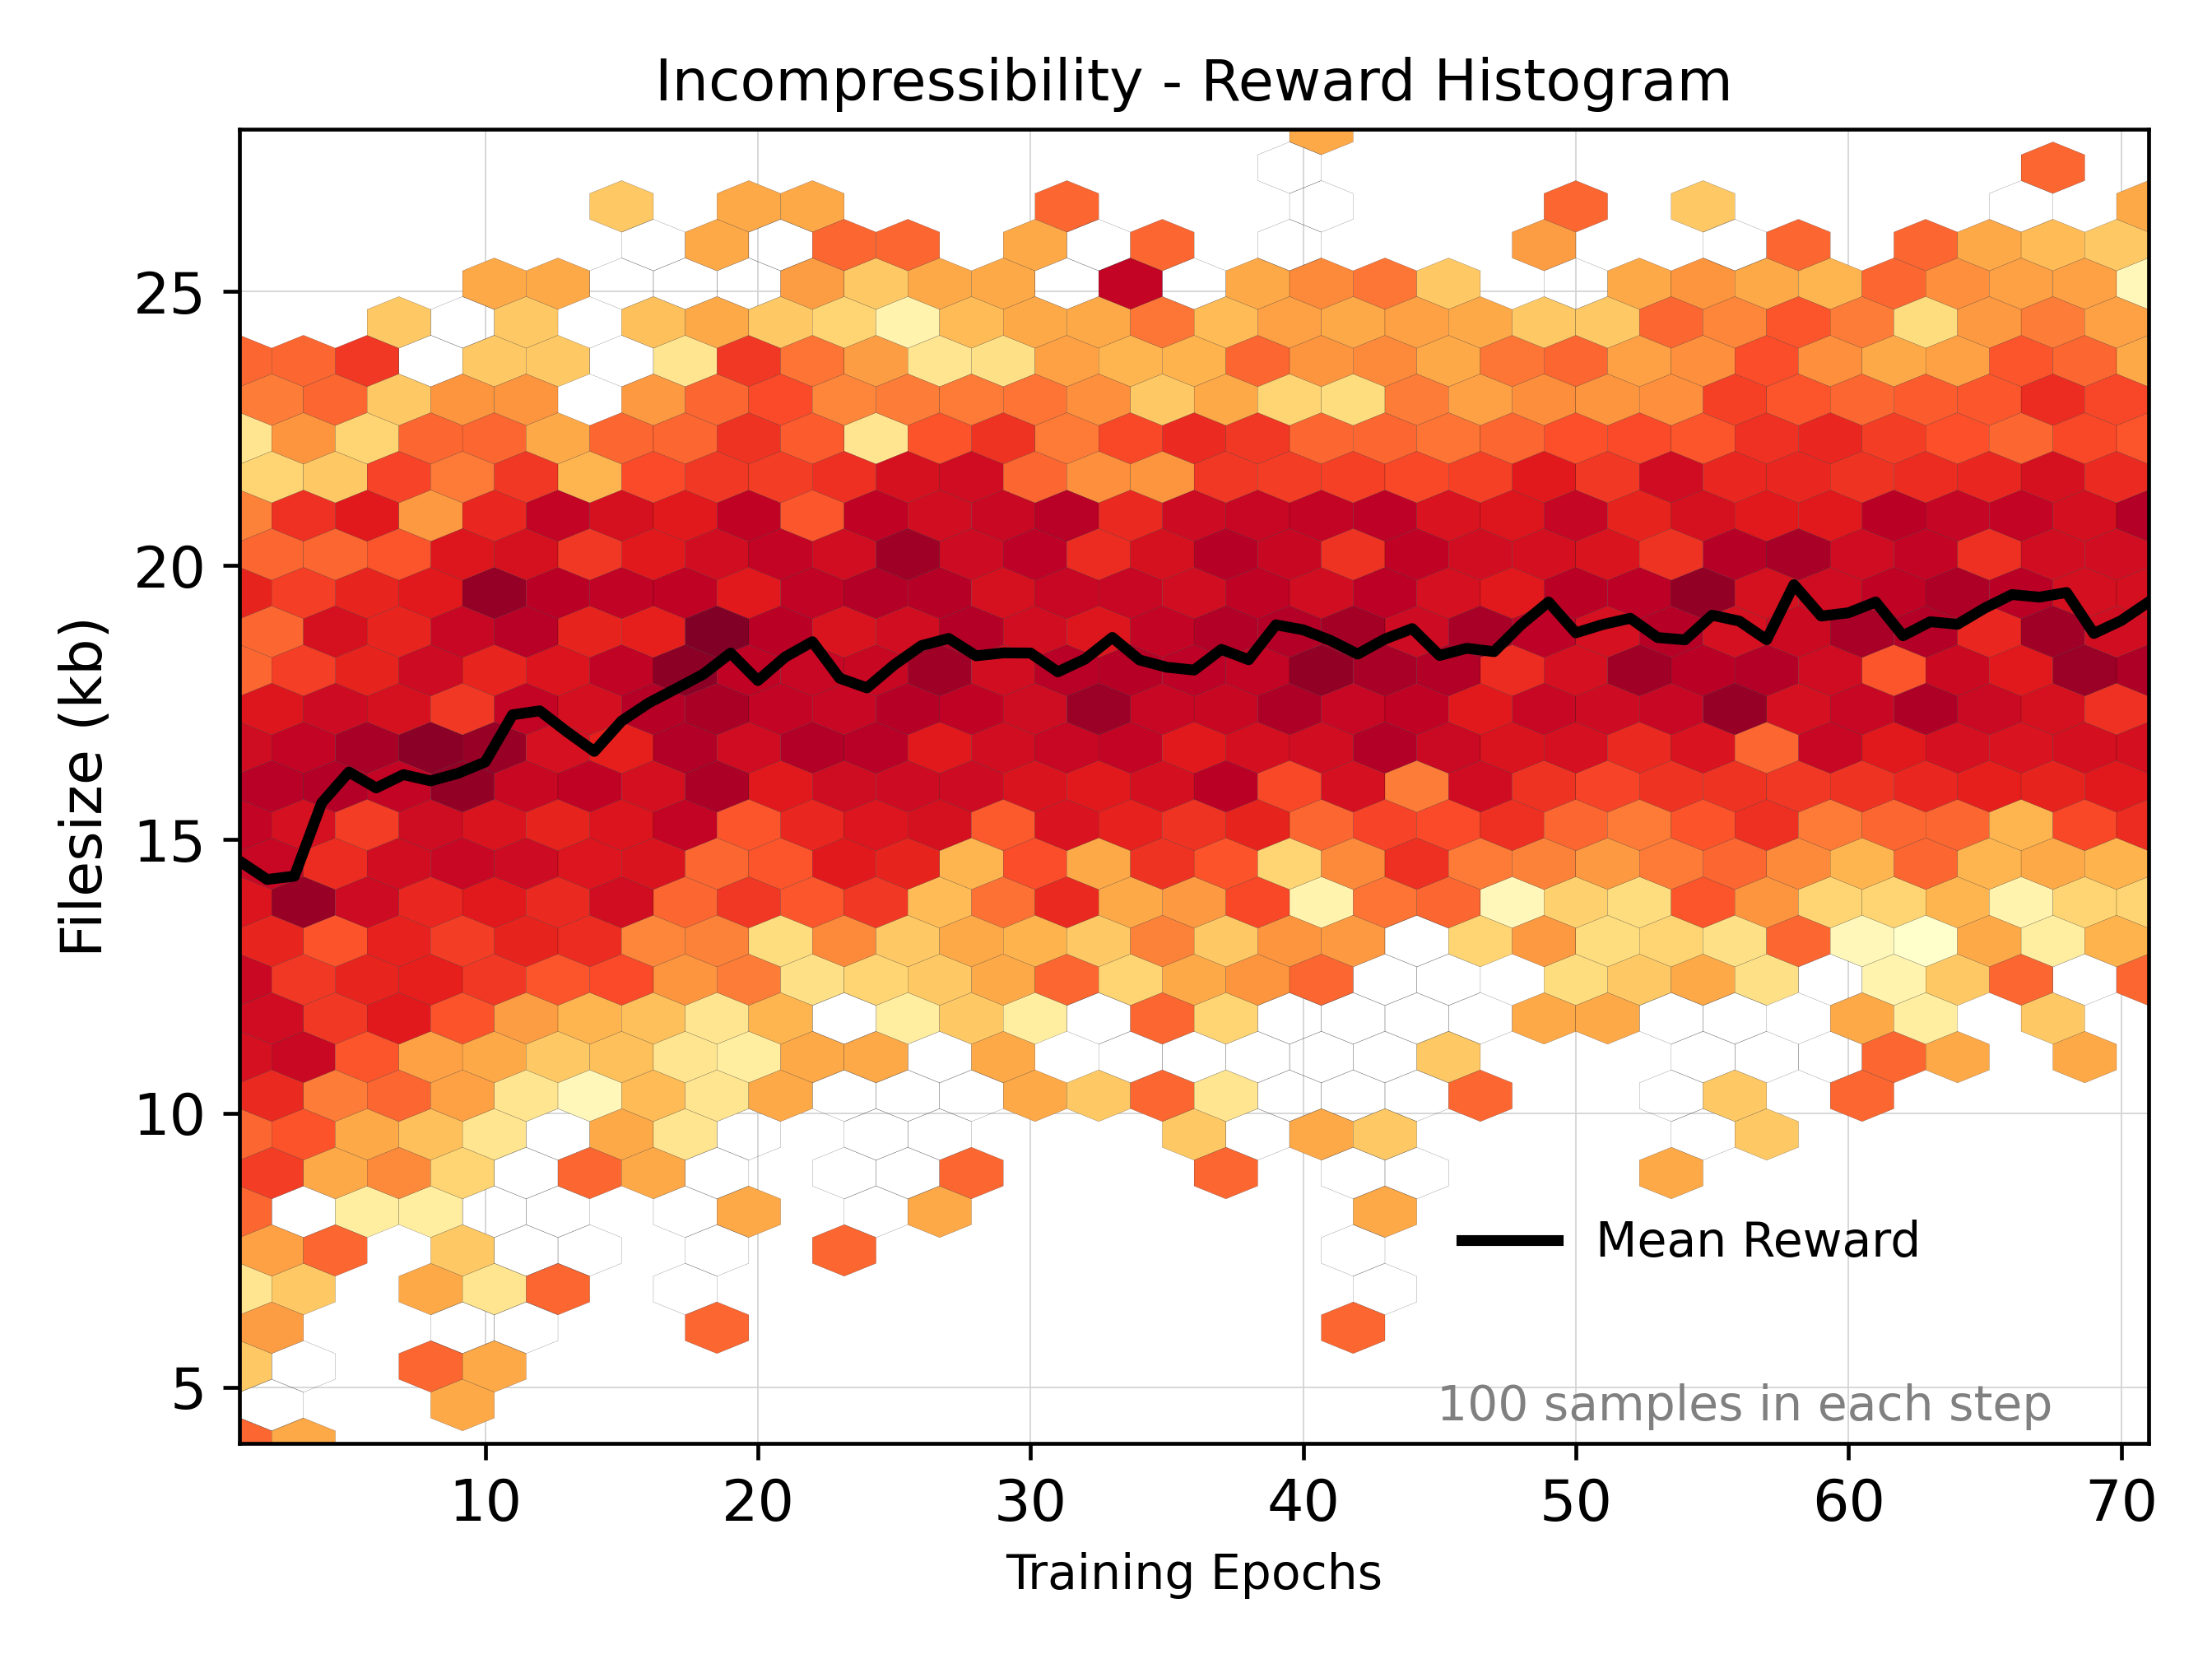
\includegraphics[width=1\textwidth]{img/results/reward_hist-jpeg-incompressibility.png} % forth figure itself
      %\label{fig:sample_figure_4}
  \end{minipage}
  \vspace{-8pt}  % reduce space between caption and figure
    \captionsetup{width=\textwidth} % set the width of the caption
    \caption{\textbf{Learning curves from DDPO.} Evolution of the mean reward (black line) and histogram during the training steps for each \textit{downstream task}. The reward estimates were computed in each step using $100$ samples from the model.}
  \label{fig:reward_hist} % Add a proper reference for the label
\end{figure}

\noindent \textbf{For JPEG compressibility and incompressibility tasks}, optimization can be achieved using a fixed learning rate ($1e-5$), resulting in smooth transitions in the image as the model parameters shift from the initial  pretrained DDPM model to the final DDPO finetuned model. This process is  illustrated in Figure~\ref{fig:ddpm-to-ddpo-compressibility} and Figure~\ref{fig:ddpm-to-ddpo-incompressibility} for each respective reward. \\

\noindent \textbf{In the case of aesthetic quality task}, the transition is more challenging, requiring a more complex learning rate dynamics to starting to maximize the aesthetic score \ca{\textbf{Agregar un gráfico de learning rate y rewards con los runs utilizados para aesthetic quality}}. The consequences of this are abrupt changes in the image's semantic at the beginning of the training, given the learning rate warmp-up that allow  to ``escape'' from the local minima of the pretrained model. Then, a half-cosine annealing allow to smooth the transition to the final model. This process is illustrate Figure~\ref{fig:ddpm-to-ddpo-aesthetic}. \\


% Transition from DDPM to DDPO samples optimized for JPEG compressibility
\begin{figure}[ht]
  \centering
  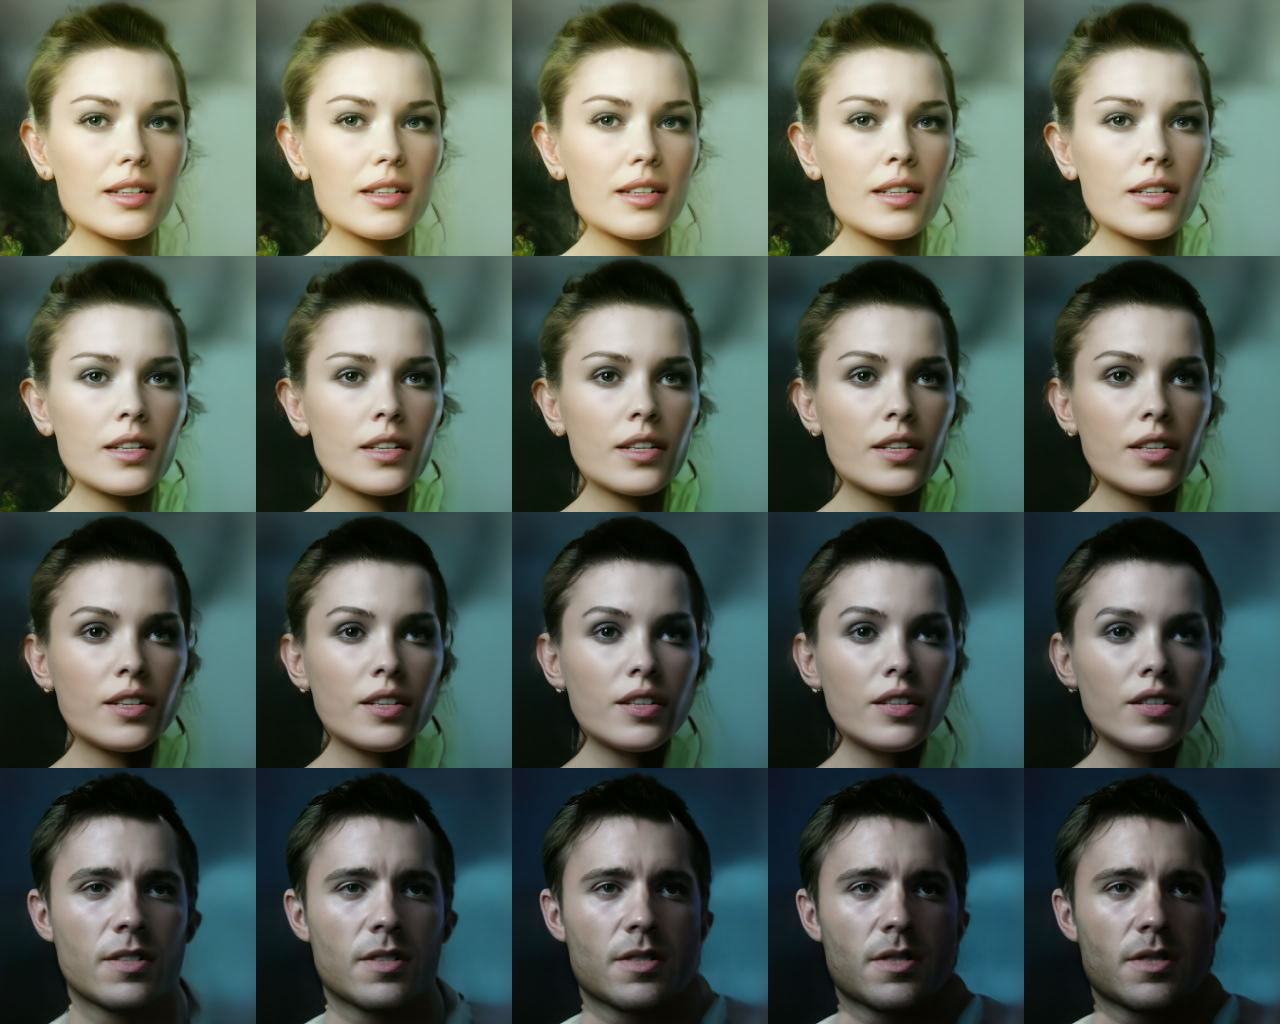
\includegraphics[scale=1.40]{img/results/compressibility_6.png}
  \vspace{-0pt}  % reduce space between caption and figure
    \captionsetup{width=\textwidth} % set the width of the caption
    \caption{\textbf{Transition from DDPM to DDPO optimized for JPEG compressibility.}}
    \label{fig:ddpm-to-ddpo-compressibility}
\end{figure}

% Transition from DDPM to DDPO samples optimized for JPEG incompressibility
\begin{figure}[ht]
  \centering
  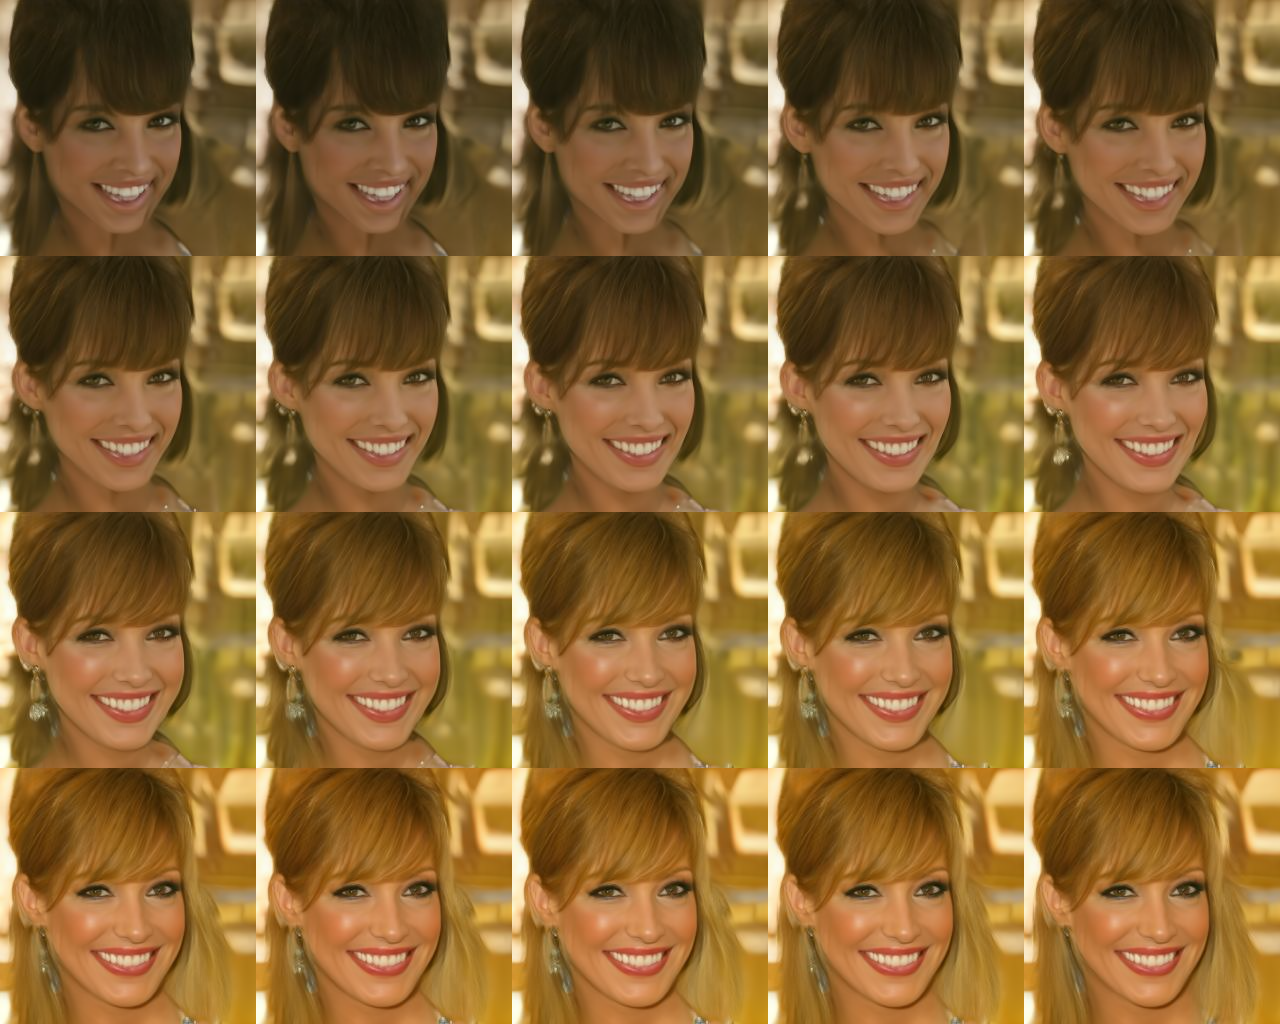
\includegraphics[scale=1.40]{img/results/incompressibility_26.png}
  \vspace{-0pt}  % reduce space between caption and figure
    \captionsetup{width=\textwidth} % set the width of the caption
    \caption{\textbf{Transition from DDPM to DDPO optimized for JPEG incompressibility.}}
    \label{fig:ddpm-to-ddpo-incompressibility}
\end{figure}

\noindent The learning dynamics for incompressibility reward are by more
difficult nature than compressibility, even when there are opposite of the
same coind. This is reflected in the reward curves during training (Figure~\ref{fig:reward_hist}). The mean reward for incompressibility. Lo que tiene sentido según la naturaleza del task y las capacidades del modelo. Hasta cierto punto, añadir mayor información  requiere de mayores capacidades generativas para agregar semantica visual y  otros features dentro de la imagen que no se pierdan durante el proceso de compresión. Sin embargo, reducir el tamaño del archivo siempre se puede alcanzar destruyendo la capacidad de generación del modelo, i.e. quitar información es más fácil que agregar/crear información.

\noindent Learning rate más bajo permite optimizar el compressibility reward, generando transiciones más suaves. A diferencia de las dificultates que presenta optimizar el LAION aeshtetic score que requiere una dinamica de learning rate más compleja para modificar features más agresivamente para lograr maximizar la ``calidad estetica''. \\

% Transition from DDPM to DDPO samples optimized for aesthetic quality
\begin{figure}[ht]
  \centering
  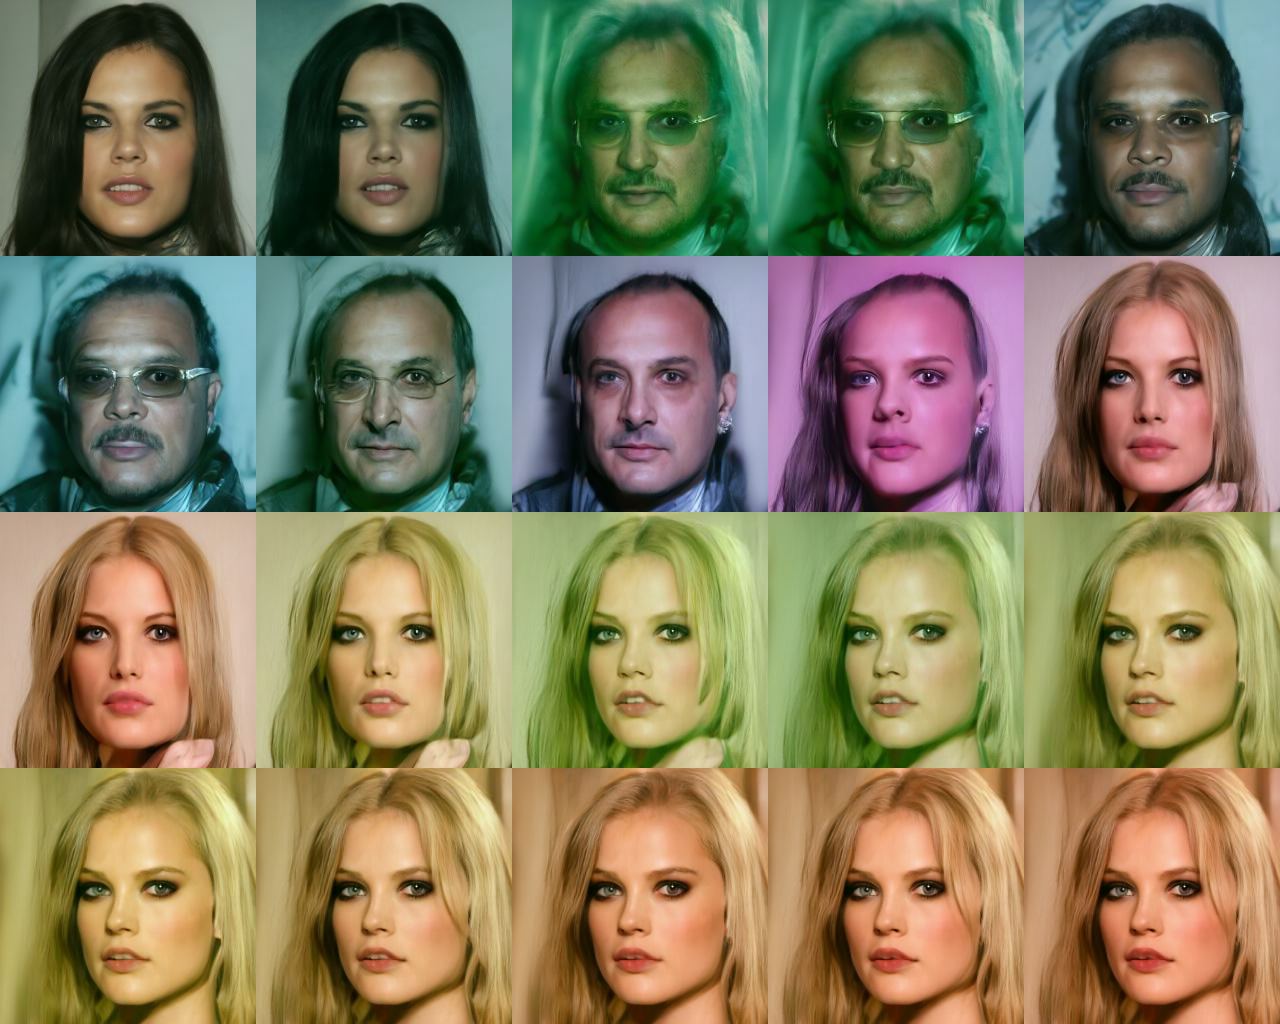
\includegraphics[scale=1.40]{img/results/laion_60.png}
  \vspace{-0pt}  % reduce space between caption and figure
    \captionsetup{width=\textwidth} % set the width of the caption
    \caption{\textbf{Transition from DDPM to DDPO optimized for aesthetic quality.}}
    \label{fig:ddpm-to-ddpo-aesthetic}
\end{figure}

\noindent \textbf{ViT Age Classifier.} Task to move the increase the sample frequency of faces over 50 years old.

% ViT age predictin distribution on ddpm-celebahq and dpoo-celebahq finetuned
% on logits
\begin{figure}[ht]
  \centering
  \begin{minipage}{0.5\textwidth}
    \centering
    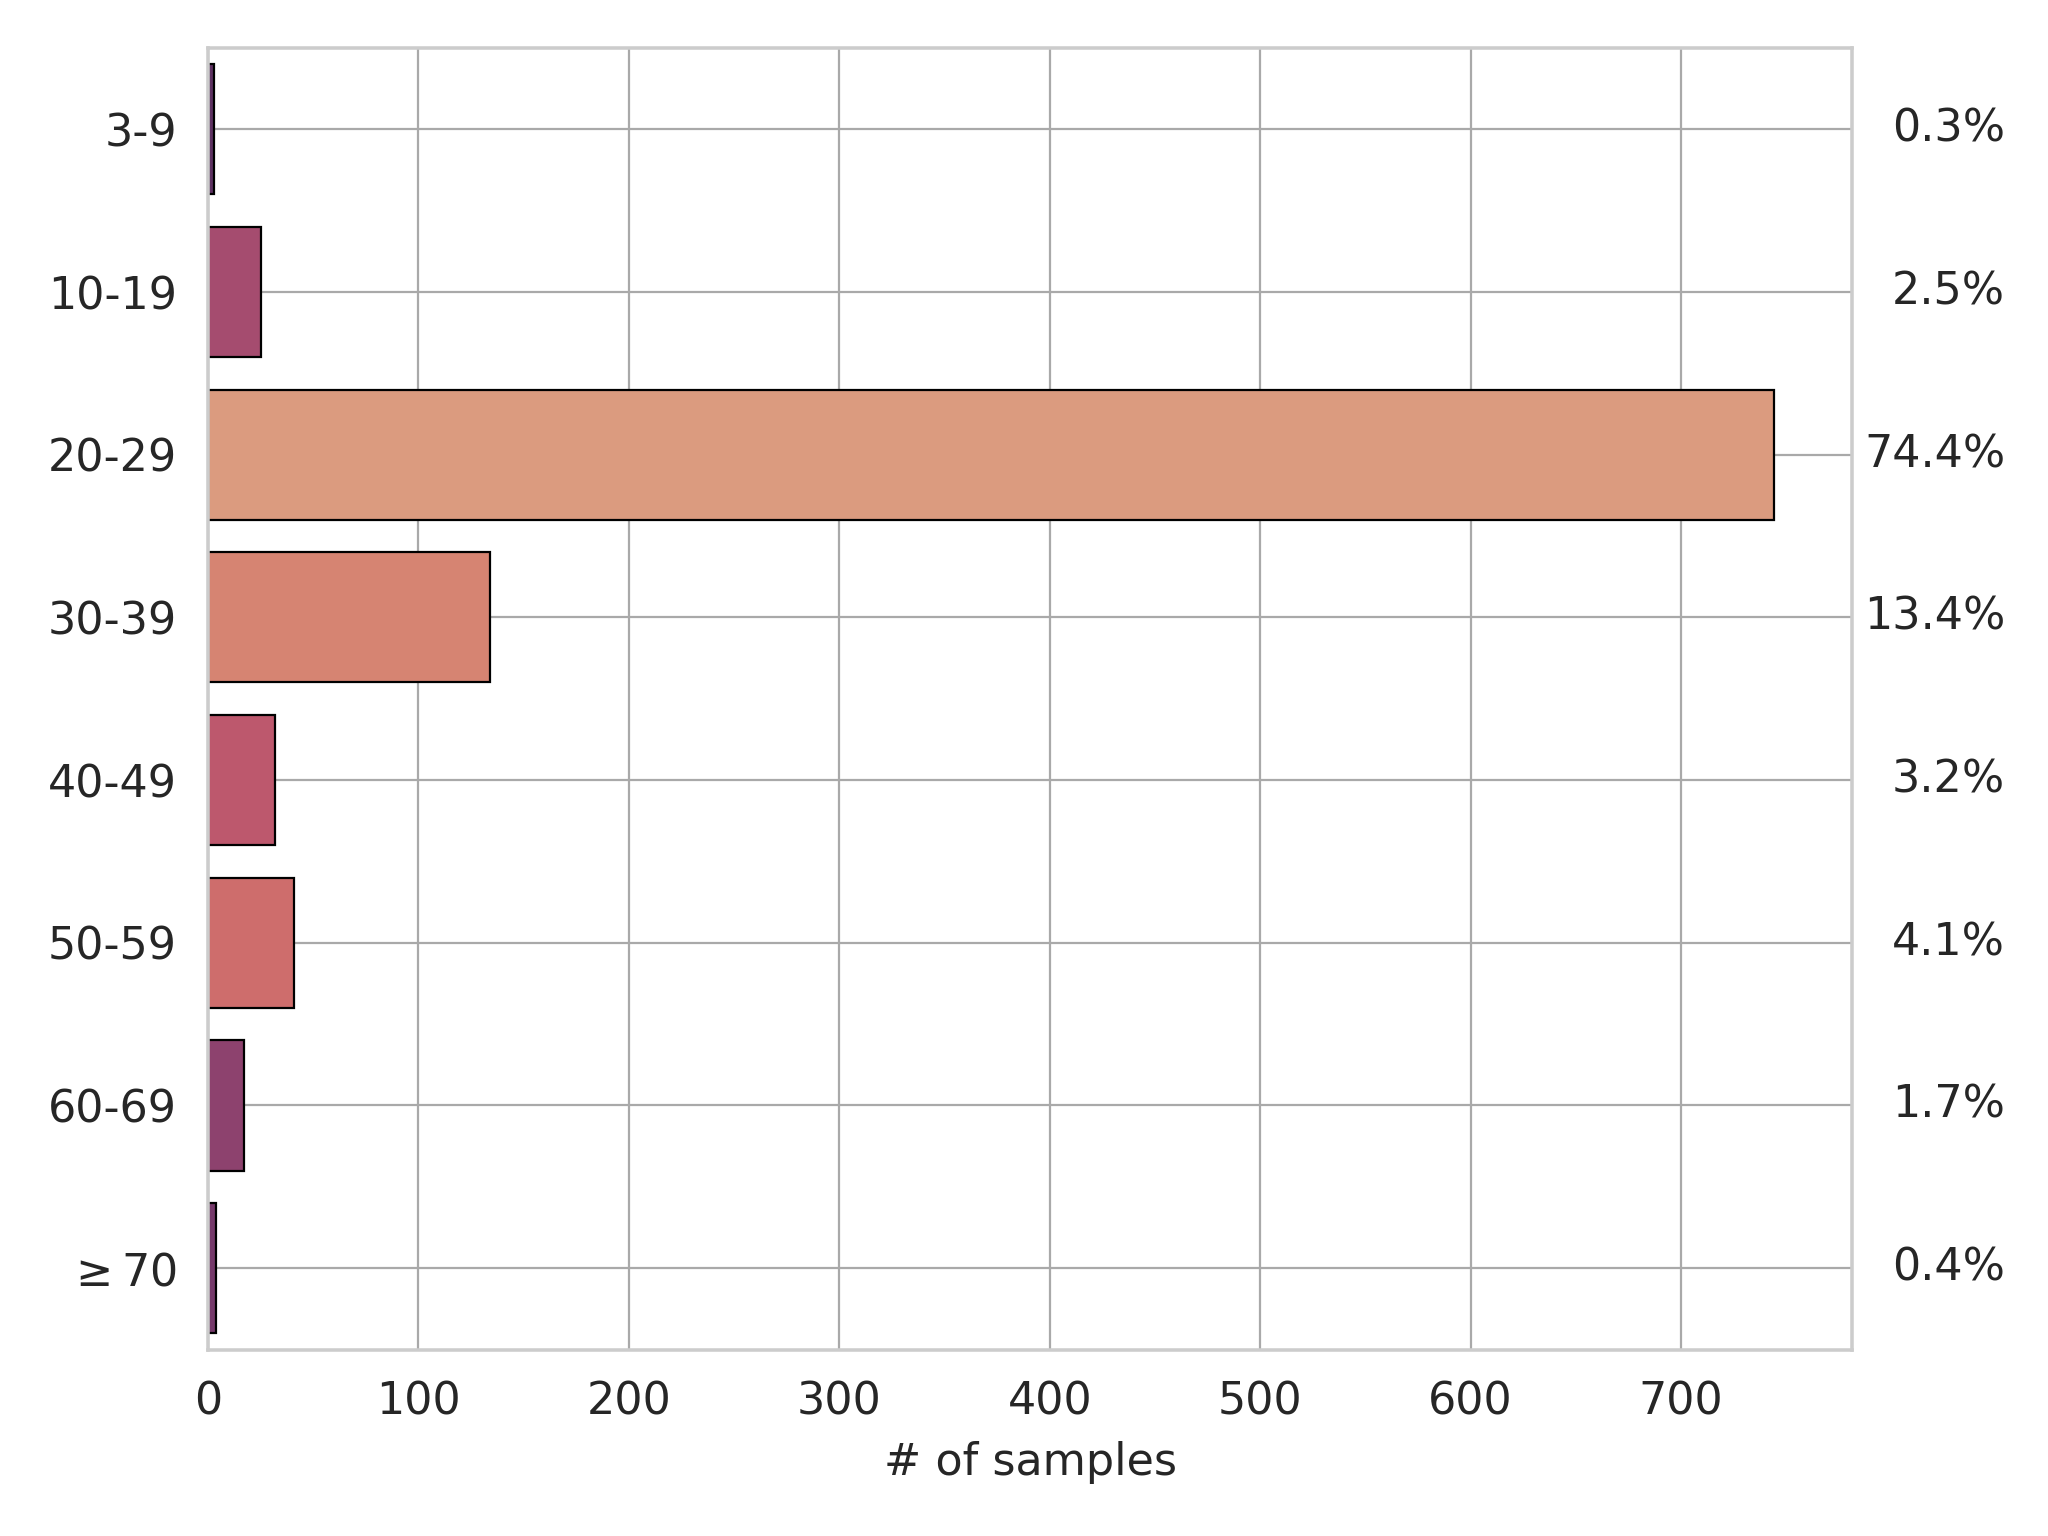
\includegraphics[width=1\textwidth]{img/results/age-dist-ddpm-celebahqsample-based-on-vit-age-preds-on-faces.png} % first figure itself
    %\label{fig:sample_figure_1}
  \end{minipage}\hfill
  \begin{minipage}{0.5\textwidth}
    \centering
    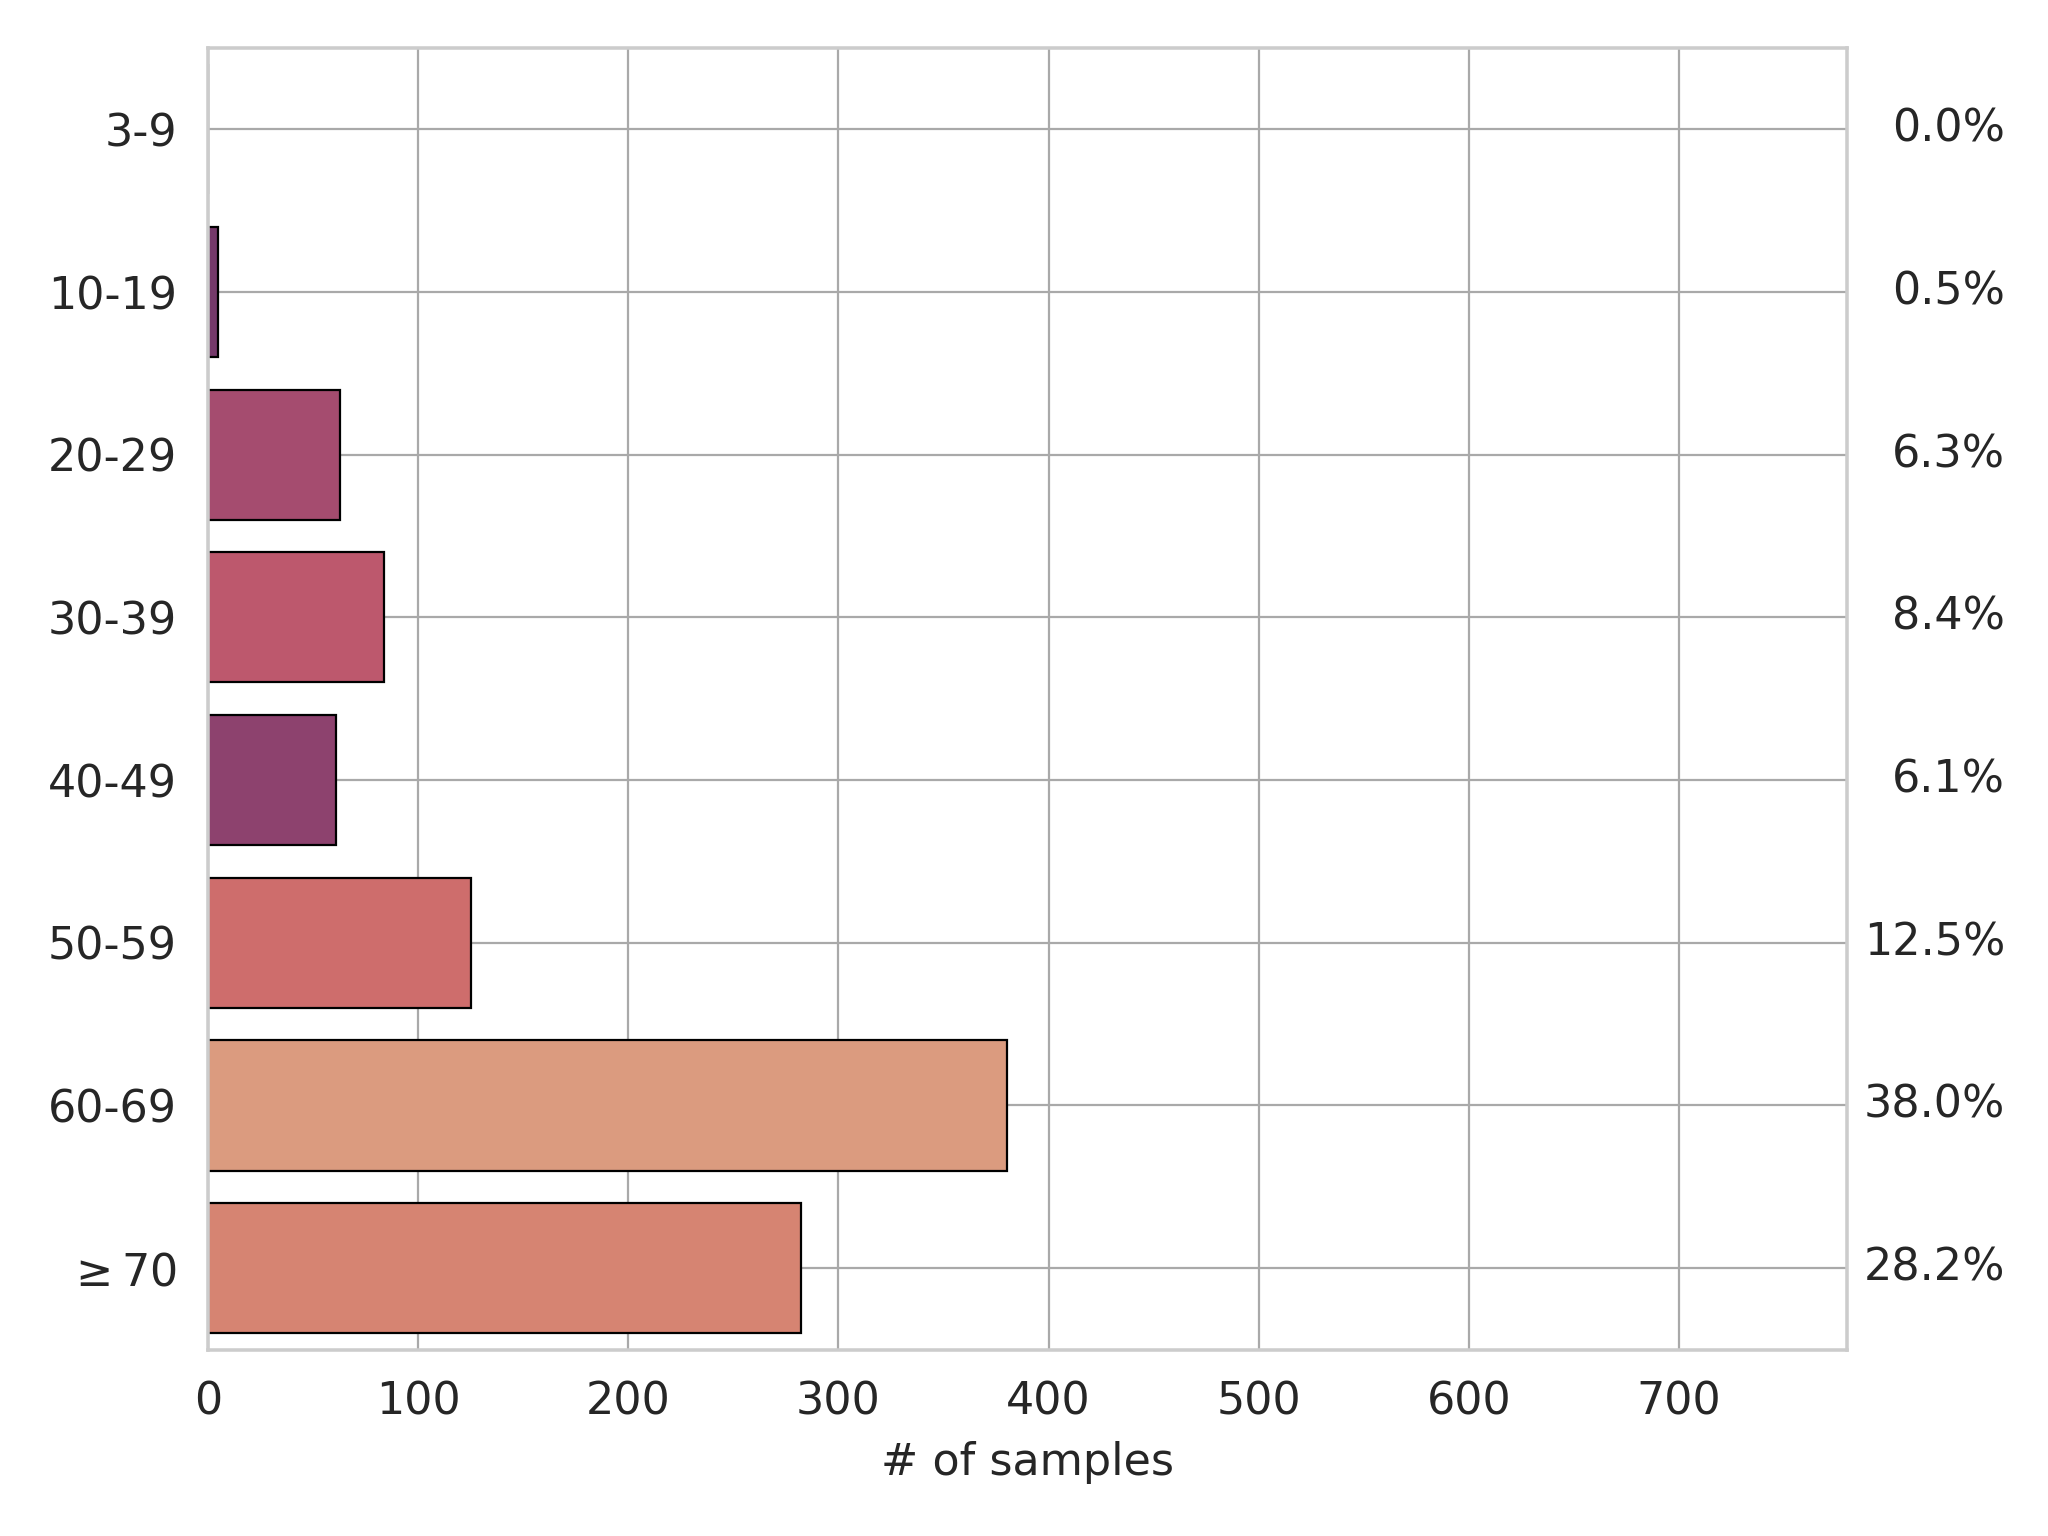
\includegraphics[width=1\textwidth]{img/results/age-dist-ddpo-celebahqsample-based-on-vit-age-preds-on-faces.png} % second figure itself
  \end{minipage}
  \vspace{-8pt}  % reduce space between caption and figure
  \captionsetup{width=\textwidth} % set the width of the caption
  \caption{\textbf{Age Distribution of Faces: Comparison Between DDPM (left) and DDPO (right).} By finetuning with DDPO to maximize the logits sum for the age classes 
  \texttt{$50-59$}, \texttt{$60-69$}, and \texttt{$\geq 70$}, we observe an increase in the proportion of faces over $50$ years old from $6.1\%$ in the baseline to $78.7\%$ in the finetuned samples.}
  \label{fig:age-face-dist} 
\end{figure}


% Transition from DDPM to DDPO samples optimized for Task.OVER50 (ViT age classifier)
\begin{figure}[ht]
  \centering
  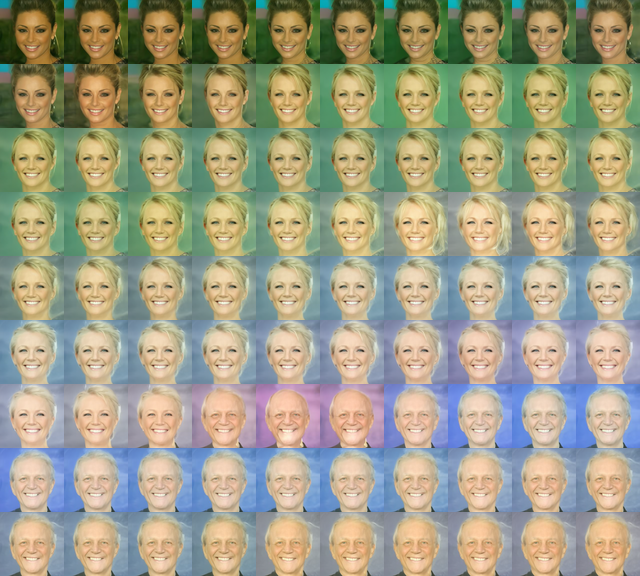
\includegraphics[scale=2.80]{img/results/over50_47.png}
  \vspace{-0pt}  % reduce space between caption and figure
    \captionsetup{width=\textwidth} % set the width of the caption
    \caption{\textbf{Transition from DDPM to DDPO optimized for over50.}}
    \label{fig:ddpm-to-ddpo-over50}
\end{figure}




\section{Discussion \& Limitations}

\noindent\textbf{Overoptimization and diversity samples.} Despite the benefits 
of optimizing diffusion models using reinforcement learning, reward overoptimization remains a significant challenge. This issue arises when the model excessively exploits the reward function \cite{gao2023scaling}, leading to a lack of diversity in the generated samples. In severe cases, this can degrade image semantics, resulting in a model that fails to achieve practical utility. \\

\noindent To understand and visualize reward overoptimization in the context of this work, we extract CLIP \cite{radford2021learning} features from two sets of images that share the
same initial seed and noise. One set is generated by the pretrained DDPM model (as mentioned in section \ref{sec:empirical-analysis}), and the other set is generated using a DDPO checkpoint optimized for aesthetic quality. We then  project these image features into a 2D embedding space using t-SNE \cite{van2008visualizing} to visualize the samples. \\

\noindent As shown in Figure~\ref{fig:clip-emb-ddpo-vs-ddpm}, we observe that the samples optimized for aesthetic quality cluster near the sample with the highest aesthetic score from the DDPM set (illustrated in Figure~\ref{fig:sample-trajectories}). This occurs because the model reinforces samples with higher aesthetic quality, generating more of these samples until the
model concentrates on a very specific high-reward region, ultimately collapsing into a single mode. \\

\noindent An intriguing research direction involves identifying and managing local features in images to unlock alternative high-reward areas. This approach helps prevent mode collapse or at least reduce its impact without compromising sample diversity. (\ca{dejo esto o lo muevo a conclusiones?}) \\
\begin{figure}[ht]
  \centering
  \includegraphics[scale=0.72]{img/results/emb-space-ddpo-vs-ddpm.png}
  \vspace{-45pt}  % reduce space between caption and figure
    \captionsetup{width=\textwidth} % set the width of the caption
    \caption{\textbf{CLIP Feature Embedding Space: DDPM vs. DDPO Samples.} Both set of samples were generated from the same seed. Notice that samples optimized for aesthetic quality reside close to the highest aesthetic score sample from the DDPM pretrained model (Figure~\ref{fig:sample-trajectories}). This is a clear example of the \textit{\textbf{mode collapse effect}}.}
    \label{fig:clip-emb-ddpo-vs-ddpm}
\end{figure}

%\noindent For visualizing the mode collapse effect, we can use the CLIP feature 
%of two set of images that share the same seed as starter point, but
%one is generated with the pretrained model and the other with a DDPO checkpoint optimized for aesthetic quality. Then we project the image features using t-SNE \cite{van2008visualizing} into a 2D embedding space in which the samples can visualize. Notice that samples from the DDPM pretrained model and the samples optimized for aesthetic quality using DDPO. The samples optimized for aesthetic quality are close to the highest aesthetic score sample from the DDPM pretrained model, which is a clear example of the mode collapse effect.\\ 


\noindent\textbf{Broader impact.} \ca{Mencionar algo sobre reproducción y exacerbación de sesgos dentro del dataset. Además del mal uso que se le pueda dar a los modelos generativos, especificamente a los de imágenes como deepfake y otros usos maliciosos. Apoyarse con citas en este trabajo..., sin embargo, mencionar también que el uso de RLHF sobre modelos generativos es una vía para el problema de alignment y ver como alinear los objetivos del modelo a valores (idealmente deseables) del operador...} Generative model trained on matching
the data distribution, as well as diffusion models. The \texttt{gogle/ddpm-celebahq-256} is a model trained on the CelebA-HQ dataset, which contains a bias for celebrity faces, it is not representative of the general population.
A potential risk is the use of the model to exarcerbate the bias in digital realm or social media, to generate fake images.

It doesn't require to pay much attention to notice that the mode collapse effect showing previously is a clear example of the preference bias suffering the reward model, the samples with higher reward are concentrate in a women, white and blond hair profiles (see more samples in Figure~\ref{fig:ddpo-aesthetic-samples}). The
use of RLHF techniques to align the model to the operator preferences is a
way to mitigate an issue, but it can also use to exacerbate the problem, or can bring unexpected consequence for align subjective objectives or preferences
that can be non representatives.\\

\noindent\textbf{Future Work.} (i) Increment the reward controling the trade-off by the overoptimization and diveristy samples. In the extreme, it is possible to unlock multiple higher reward zones to avoid collapsing to the mode? (ii) Make the intermediate reward signal estimation more robust coupling with the value function (see MaDI works). (iii) The exploration of DDPO is
fairly simple, sampling images in each iteration. Can we take advatange of intermediate states to explore the space more efficiently? Introduce an agent that can build intermediate denoised modifications that worth to explore in order to increase the data generated in a useful way for the DDPO or an alternative preference algorithms.
